\documentclass[11pt, a4paper]{article}
%\usepackage{proj1}
\usepackage{natbib}
\usepackage{fancyhdr}  
\usepackage{subcaption}
\usepackage{caption}
\usepackage{graphicx}
\usepackage{numprint}
\usepackage{multirow}
\linespread{1.25} 
\setlength{\parindent}{0cm}
\graphicspath{{Images/}}
\usepackage{hyperref}
\usepackage{amsmath}
\usepackage{amsfonts}
\usepackage{amssymb}
\usepackage{amsthm}
\usepackage{mathtools}
\usepackage{commath}
\usepackage{bbm}

%\usepackage[sc,osf]{mathpazo}
\usepackage{subcaption}
\usepackage[a4paper, top=1in, left=1.0in, right=1.0in, bottom=1in, includehead, includefoot]{geometry} %Usually have top as 1in

\usepackage{listings}
\usepackage{color} %red, green, blue, yellow, cyan, magenta, black, white
\definecolor{mygreen}{RGB}{28,172,0} % color values Red, Green, Blue
\definecolor{mylilas}{RGB}{170,55,241}


\hypersetup{colorlinks,linkcolor={black},citecolor={blue},urlcolor={black}}
\usepackage{color}
\urlstyle{same}


\theoremstyle{definition}
\newtheorem{definition}{Definition}[section]

%\newcommand{\Sta}{\rho}
\newcommand{\adja}{q_a}
\newcommand{\adjb}{q_b}
\newcommand{\adjaB}{q_{a,\partial \Omega}}
\newcommand{\adjbB}{q_{b,\partial \Omega}}
%\newcommand{\Con}{u}
\newcommand{\ra}{\rho_a}
\newcommand{\rb}{\rho_b}
\newcommand{\w}{\mathbf{w}}
\newcommand{\Stav}{\mathbf{v}}
\newcommand{\Adja}{\mathbf{p}}
\newcommand{\Adjb}{q}
\newcommand{\Adjc}{{p}_{\partial \Sigma}}
\newcommand{\Con}{\mathbf{f}}
\newcommand{\n}{\mathbf{n}}
\newcommand{\h}{\mathbf{h}}
\newcommand{\K}{\mathbf{K}}


\pagenumbering{gobble}
\begin{document}
	\section*{Optimization involving the inertial equations}
	\begin{align*}
	&\min_{\rho,\Stav,\mathbf{w} } \mathcal J(\rho,\Stav) \coloneqq \quad \frac{1}{2}||\rho - \widehat \rho||_{L_2(\Sigma)}^2  +\frac{\beta}{2}||\mathbf{w}||_{L_2(\Sigma)}^2\\
	&\text{subject to:}\\
	& \frac{\partial \Stav}{\partial t}= -  (\Stav \cdot \nabla)\Stav - \gamma  \Stav + \frac{\eta}{m} \nabla^2 \Stav  -\frac{1}{m}\Con +\frac{1}{m}\mathbf{w} -\frac{1}{m} \nabla V_{ext} - \frac{1}{m}\nabla \ln \rho  -\frac{1}{m}\int_\Omega \rho(r') \mathbf{K}(r,r')dr' \\
	&\frac{\partial \rho}{\partial t} + \nabla \cdot (\rho \Stav)=0 \qquad\qquad \qquad\qquad\qquad\quad \quad\quad\qquad \qquad\qquad \qquad\qquad\qquad\quad \qquad\quad\ \ \text{in} \quad \Sigma\\
	\\
	&\rho \Stav \cdot \mathbf{n} =0\qquad\qquad \qquad\qquad\qquad\qquad\qquad\qquad\qquad \qquad\qquad \qquad\qquad\qquad \qquad\qquad\quad  \text{on} \quad \partial  \Omega\\
	& \rho(r,0)=\rho_0\\
	& \Stav(r,0)=\Stav_0.
	\end{align*}
	
	\section{Example 1}
	We start with the following configurations:
	\begin{align*}
	&\rho_0 = \frac{1}{2.5321}\exp(-\sin(\pi y))\\
	&\w = \mathbf{0}\\
	&\mathbf{f} = 0.5\sin(\pi y)\\
	&\widehat \rho = \frac{1}{2.5321}\exp(-\sin(\pi y))\\
	&V_{ext} =  \sin(\pi y).
	\end{align*}
	If the imposed flow $\mathbf{f}$ was zero, this would be a steady state, since $\rho_0 = a e^{-V_{ext}}$, which is confirmed when running the problem with those configurations. The algorithm converges within one iteration in this case.\\
	The problem is therefore asking, how do we get to the steady state by applying $\w$, when we have a non-zero $\mathbf f$. We expect $\w$ to work against $\mathbf{f}$.
	We choose $n = 20$ and $N = 30$, tolerances $10^{-8}/10^{-4}$ and $\beta = 10^{-3}$. 
	
	First, we set $\gamma = 1$, $\eta = 0.1$ and $\kappa = 0$. We get that $J_{FW} = 0.0030$ and $J_{Opt} = 5.8783 \times 10^{-5}$, see Figure \ref{F1}.
	\begin{figure}[h]
		\centering
		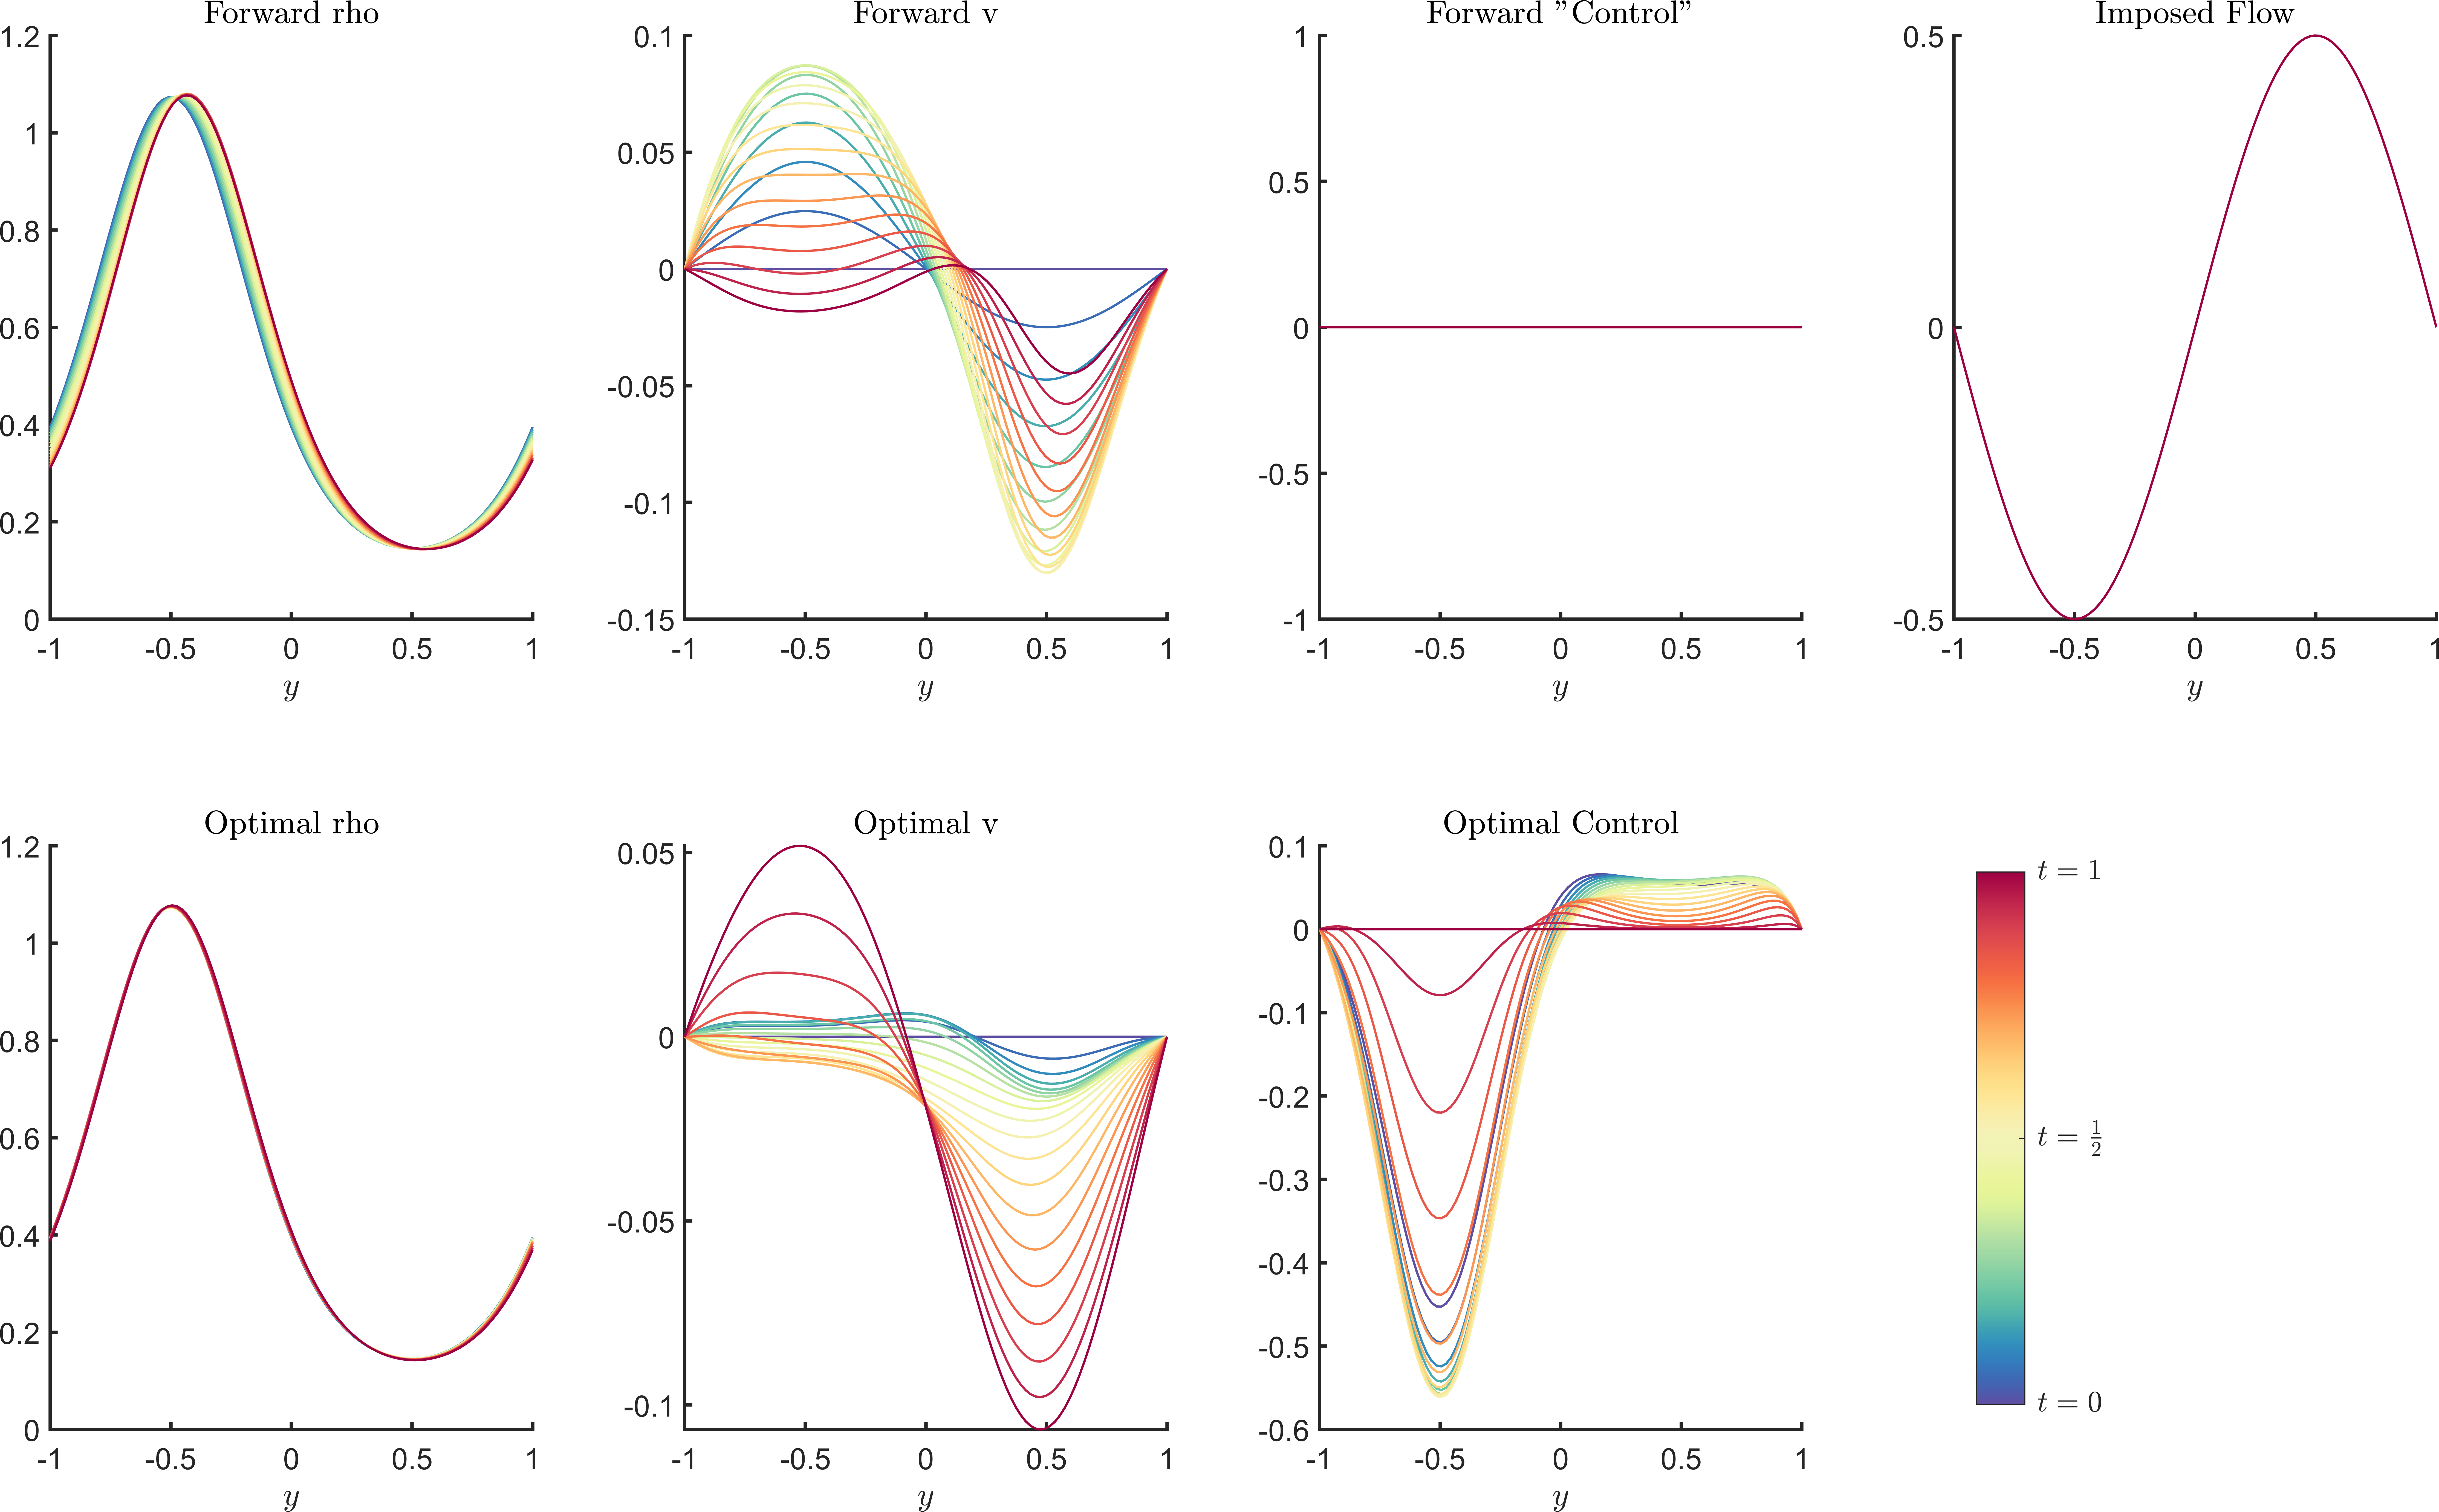
\includegraphics[scale=0.04]{Example1.png}
		\caption{Example 1, $\eta = 0.1$, $\gamma = 1$, $\kappa = 0$} 
		\label{F1}
	\end{figure}
    Then we choose $\kappa = 1$, which gives $J_{FW} = 0.0017$ and $J_{Opt} = 4.2062 \times 10^{-5}$. In Figure \ref{F1a} it can be seen that this results in differences in the dynamic. 
    For $\kappa = -1$, we get $J_{FW} = 0.0070$, $J_{Opt} = 1.5997 \times 10^{-4}$, which can be seen in Figure \ref{F1b}. While the dynamics for repulsive particles ($\kappa = 1$) are very different from the non-interacting case, the similarities between non-interacting and attractive case are quite large.
\begin{figure}[h]
	\centering
	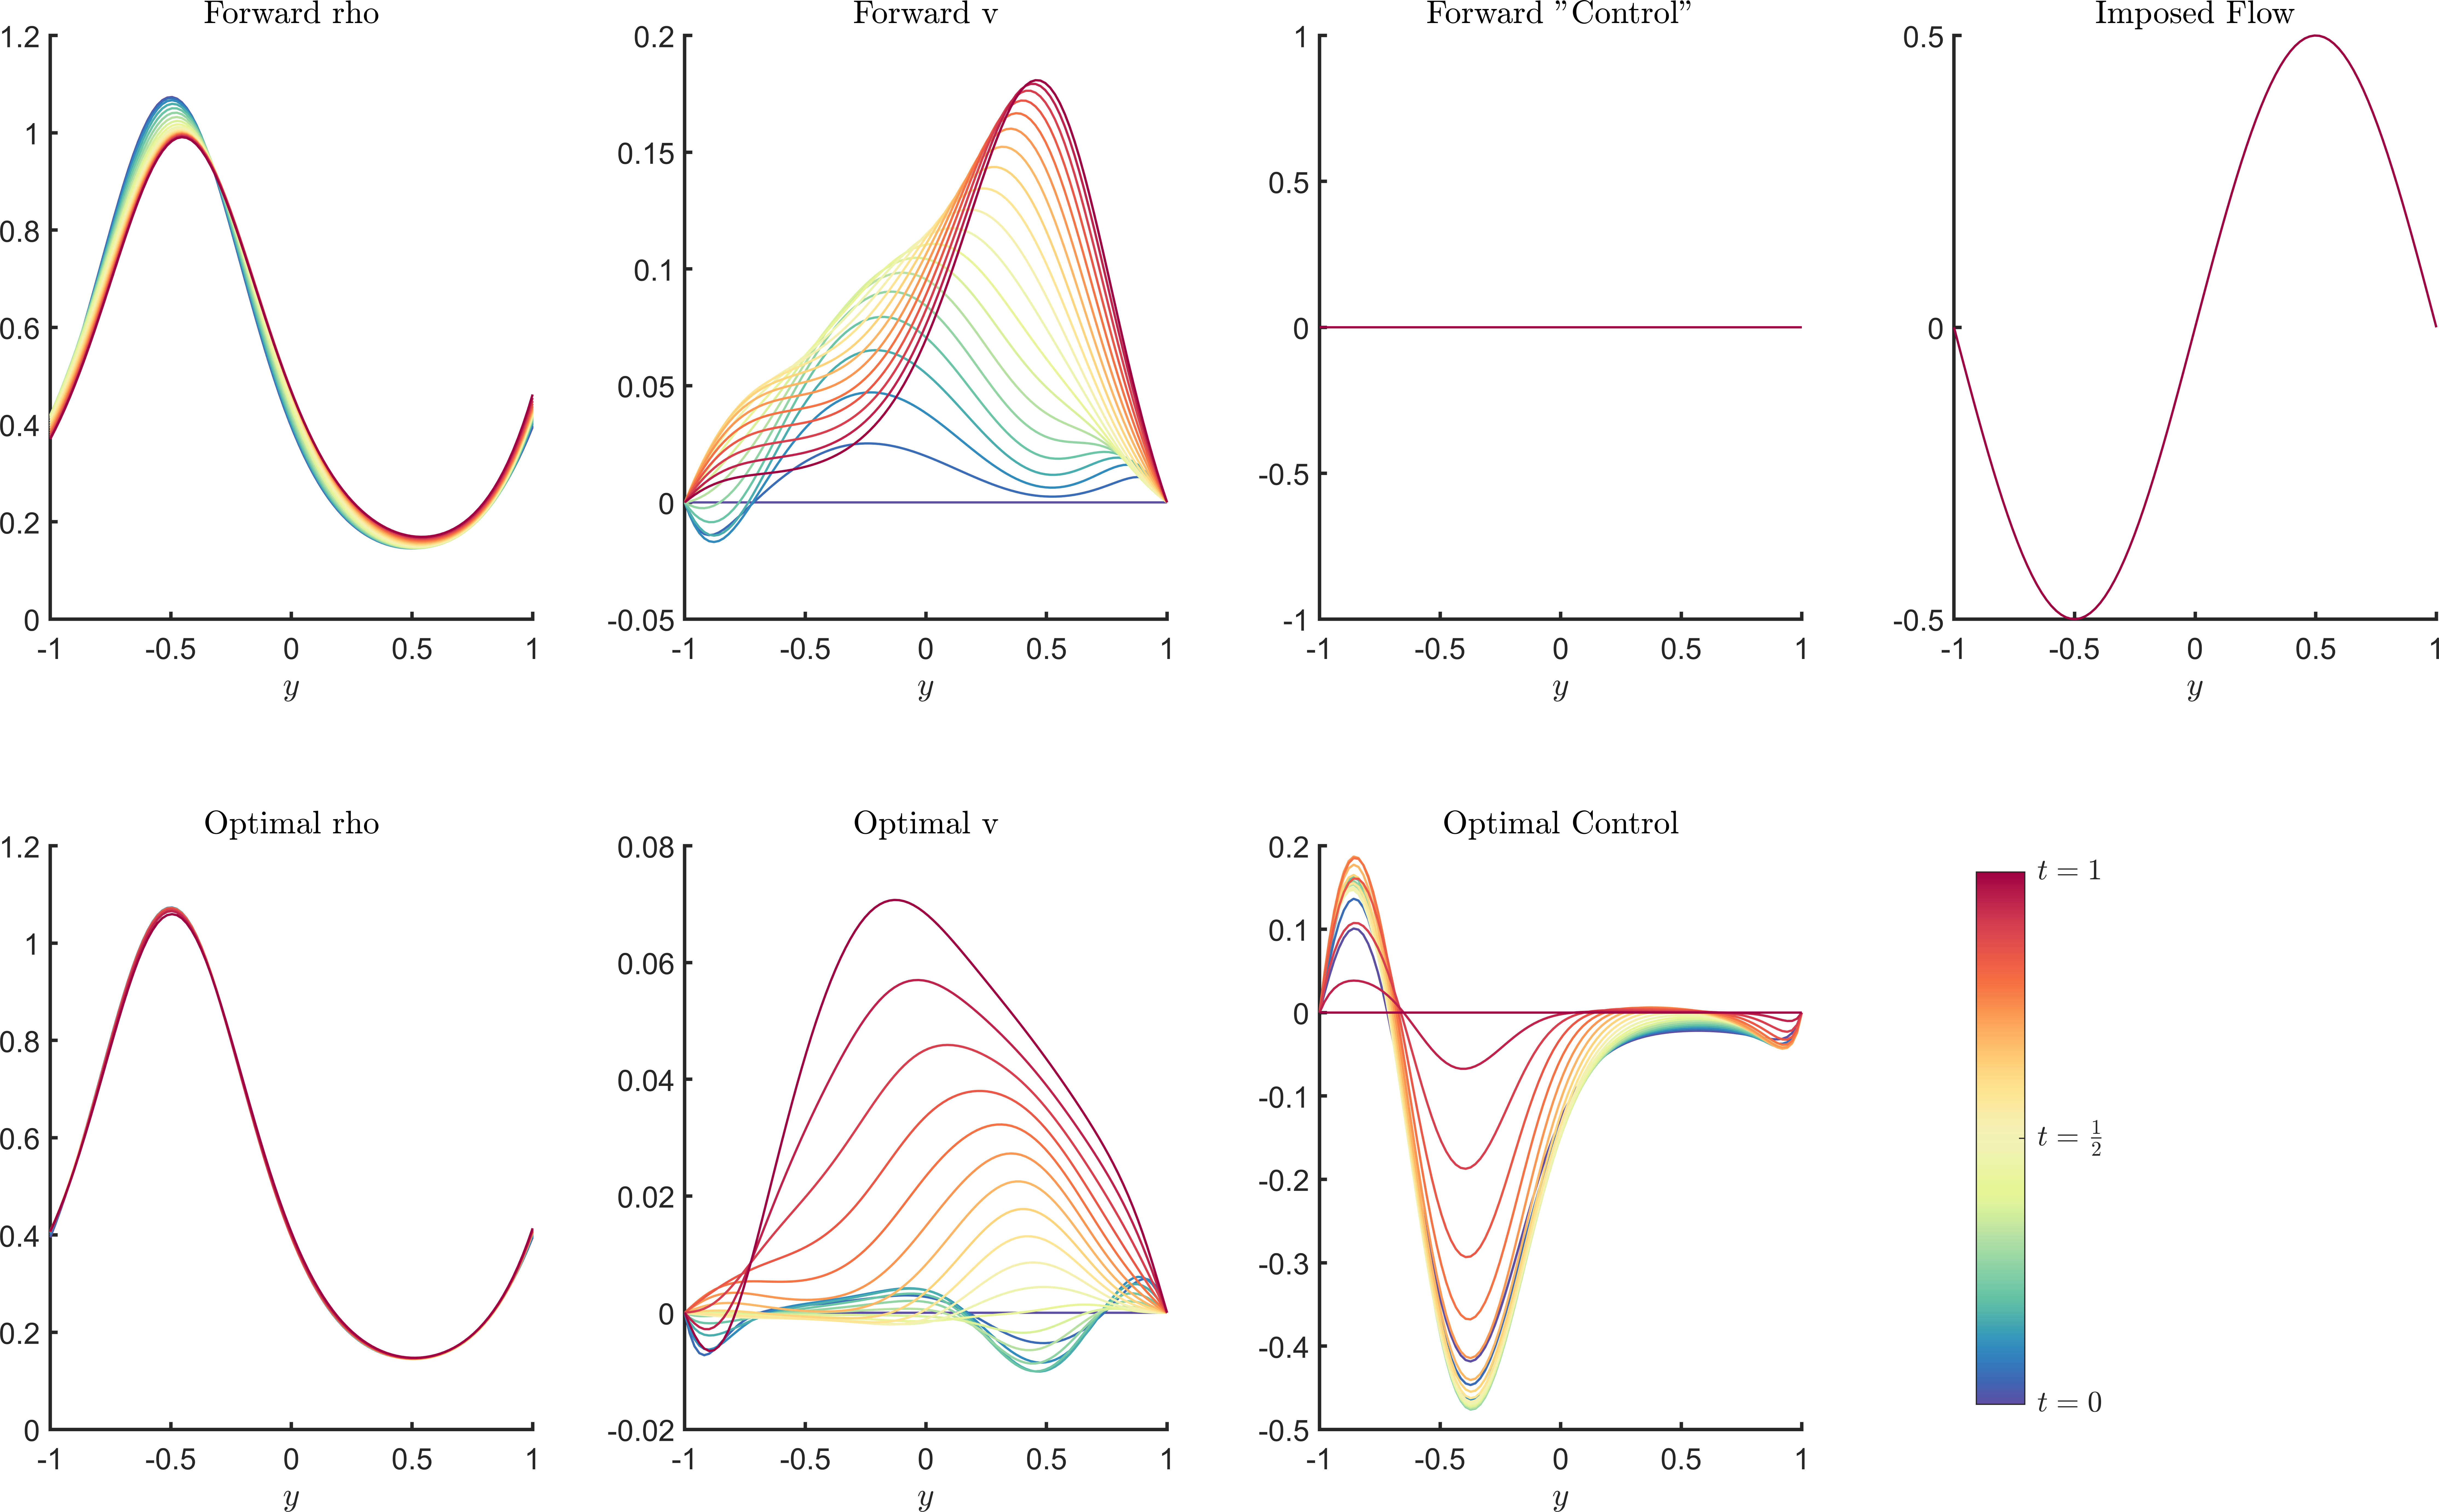
\includegraphics[scale=0.04]{Example111.png}
	\caption{Example 1, $\eta = 0.1$, $\gamma = 1$, $\kappa = 1$} 
	\label{F1a}
\end{figure}
\begin{figure}[h]
	\centering
	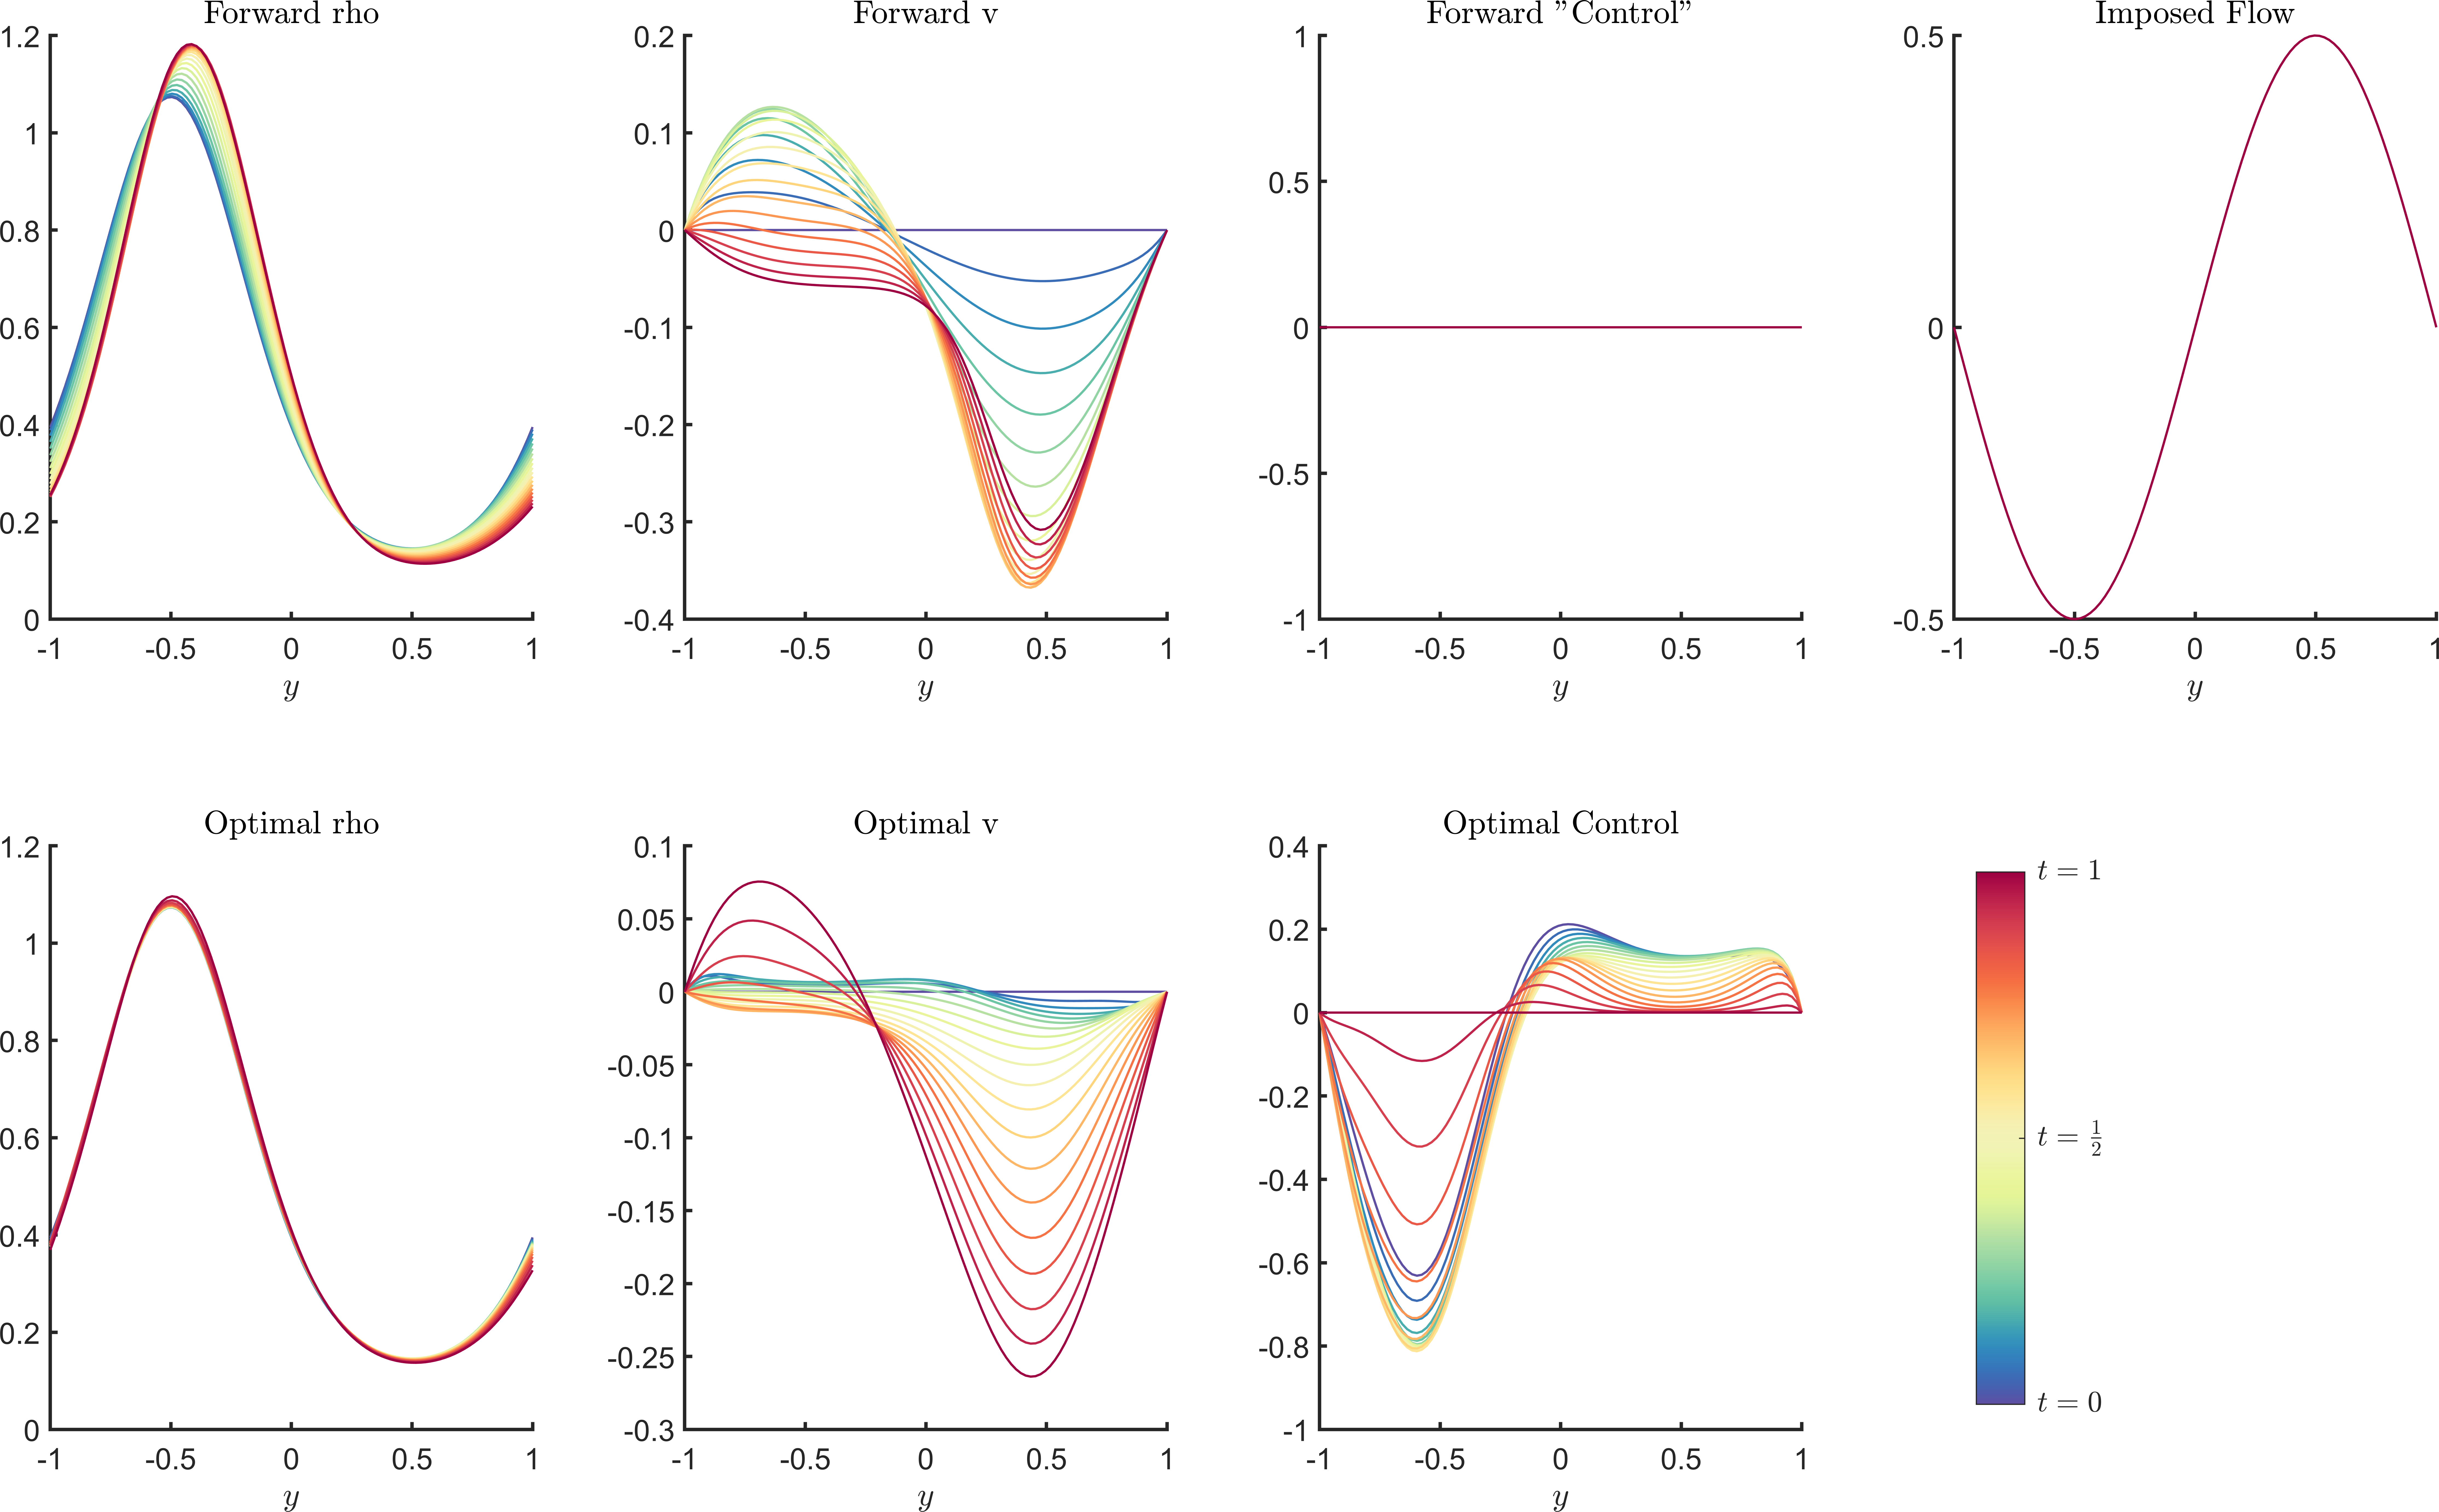
\includegraphics[scale=0.04]{Example11n1.png}
	\caption{Example 1, $\eta = 0.1$, $\gamma = 1$, $\kappa = -1$} 
	\label{F1b}
\end{figure}
	If we set $\eta = 0.01$ we get $J_{FW} = 0.0036$ and $J_{opt} = 5.7714 \times 10^{-5}$ with a very similar looking result.
	If we set $\eta = 1$ we get $J_{FW} = 7.2684 \times 10^{-4}$ and $J_{opt} = 5.5577 \times 10^{-5}$, and the forward problem is much closer to our steady state already, due to the high value of the smoothing term, see Figure \ref{F2}.
	\begin{figure}[h]
		\centering
		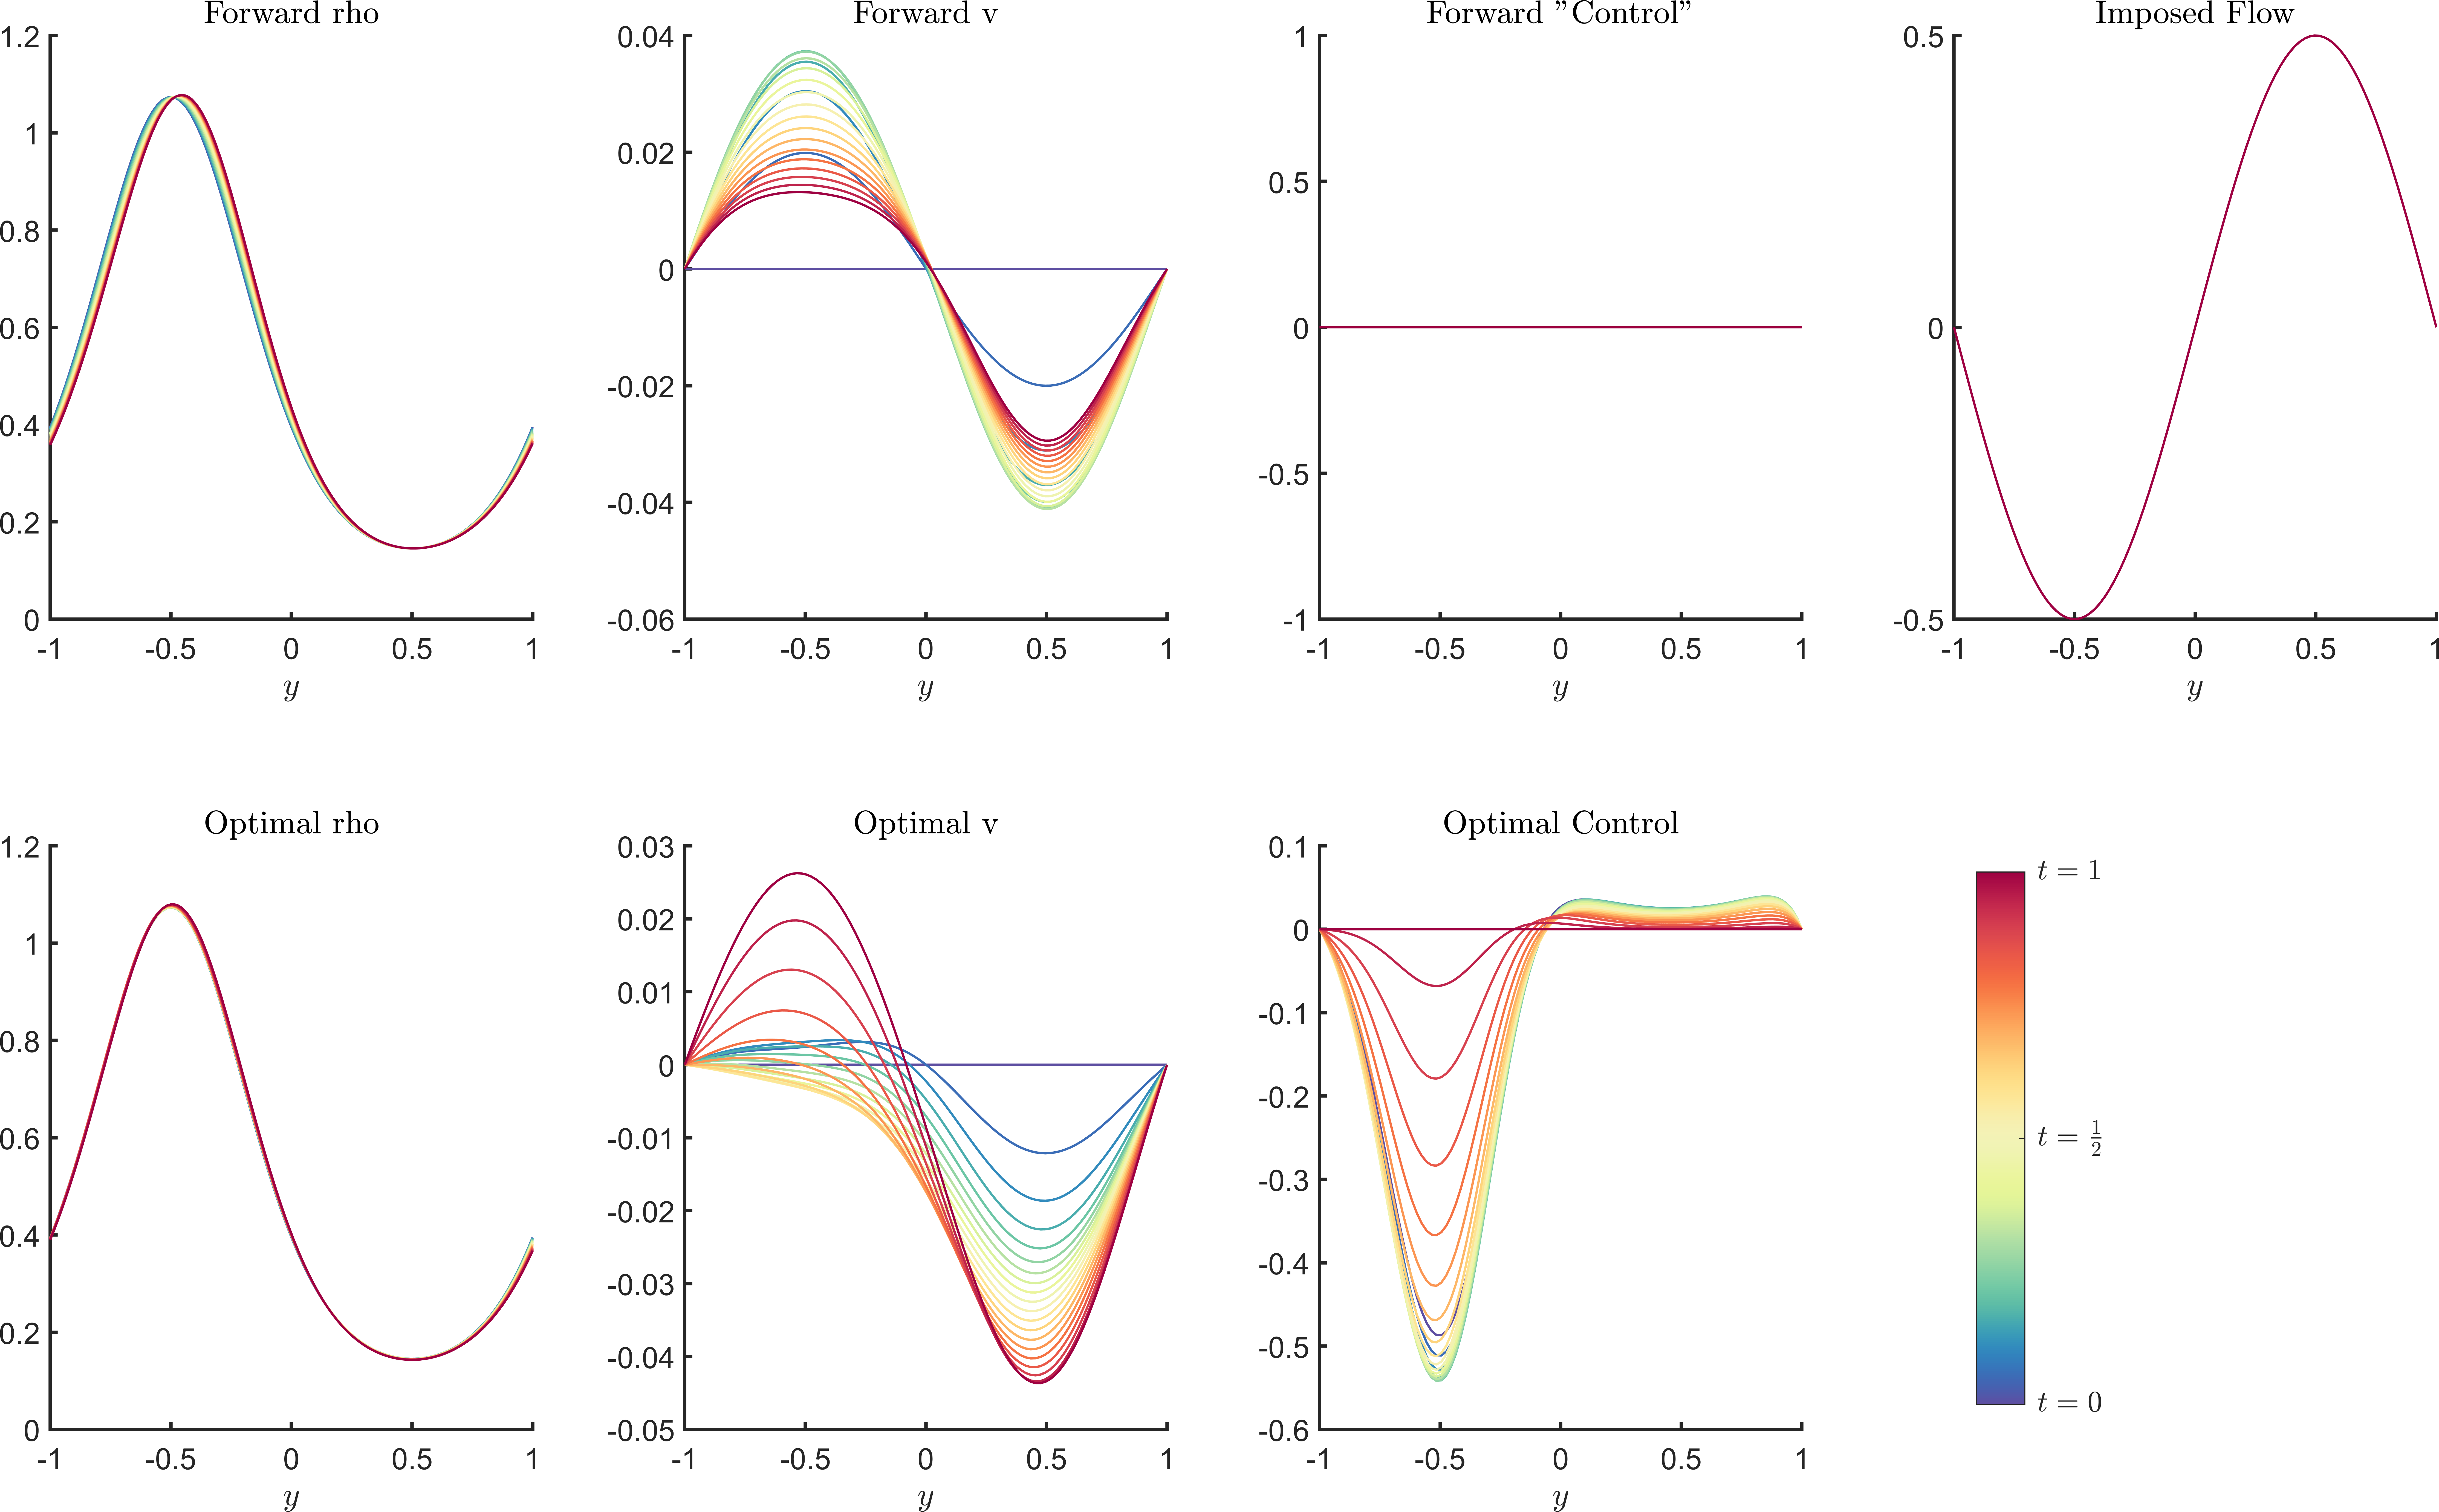
\includegraphics[scale=0.04]{Example1a.png}
		\caption{Example 1, $\eta = 1$, $\gamma = 1$, $\kappa = 0$} 
		\label{F2}
	\end{figure}
	Choosing instead $\gamma = 10$ and $\eta = 0.1$, we again start closer to $\widehat \rho$. We get $J_{FW} = 6.3845 \times 10^{-4}$, $J_{Opt} = 5.7124 \times 10^{-5}$, see Figure \ref{F3}.
	\begin{figure}[h]
		\centering
		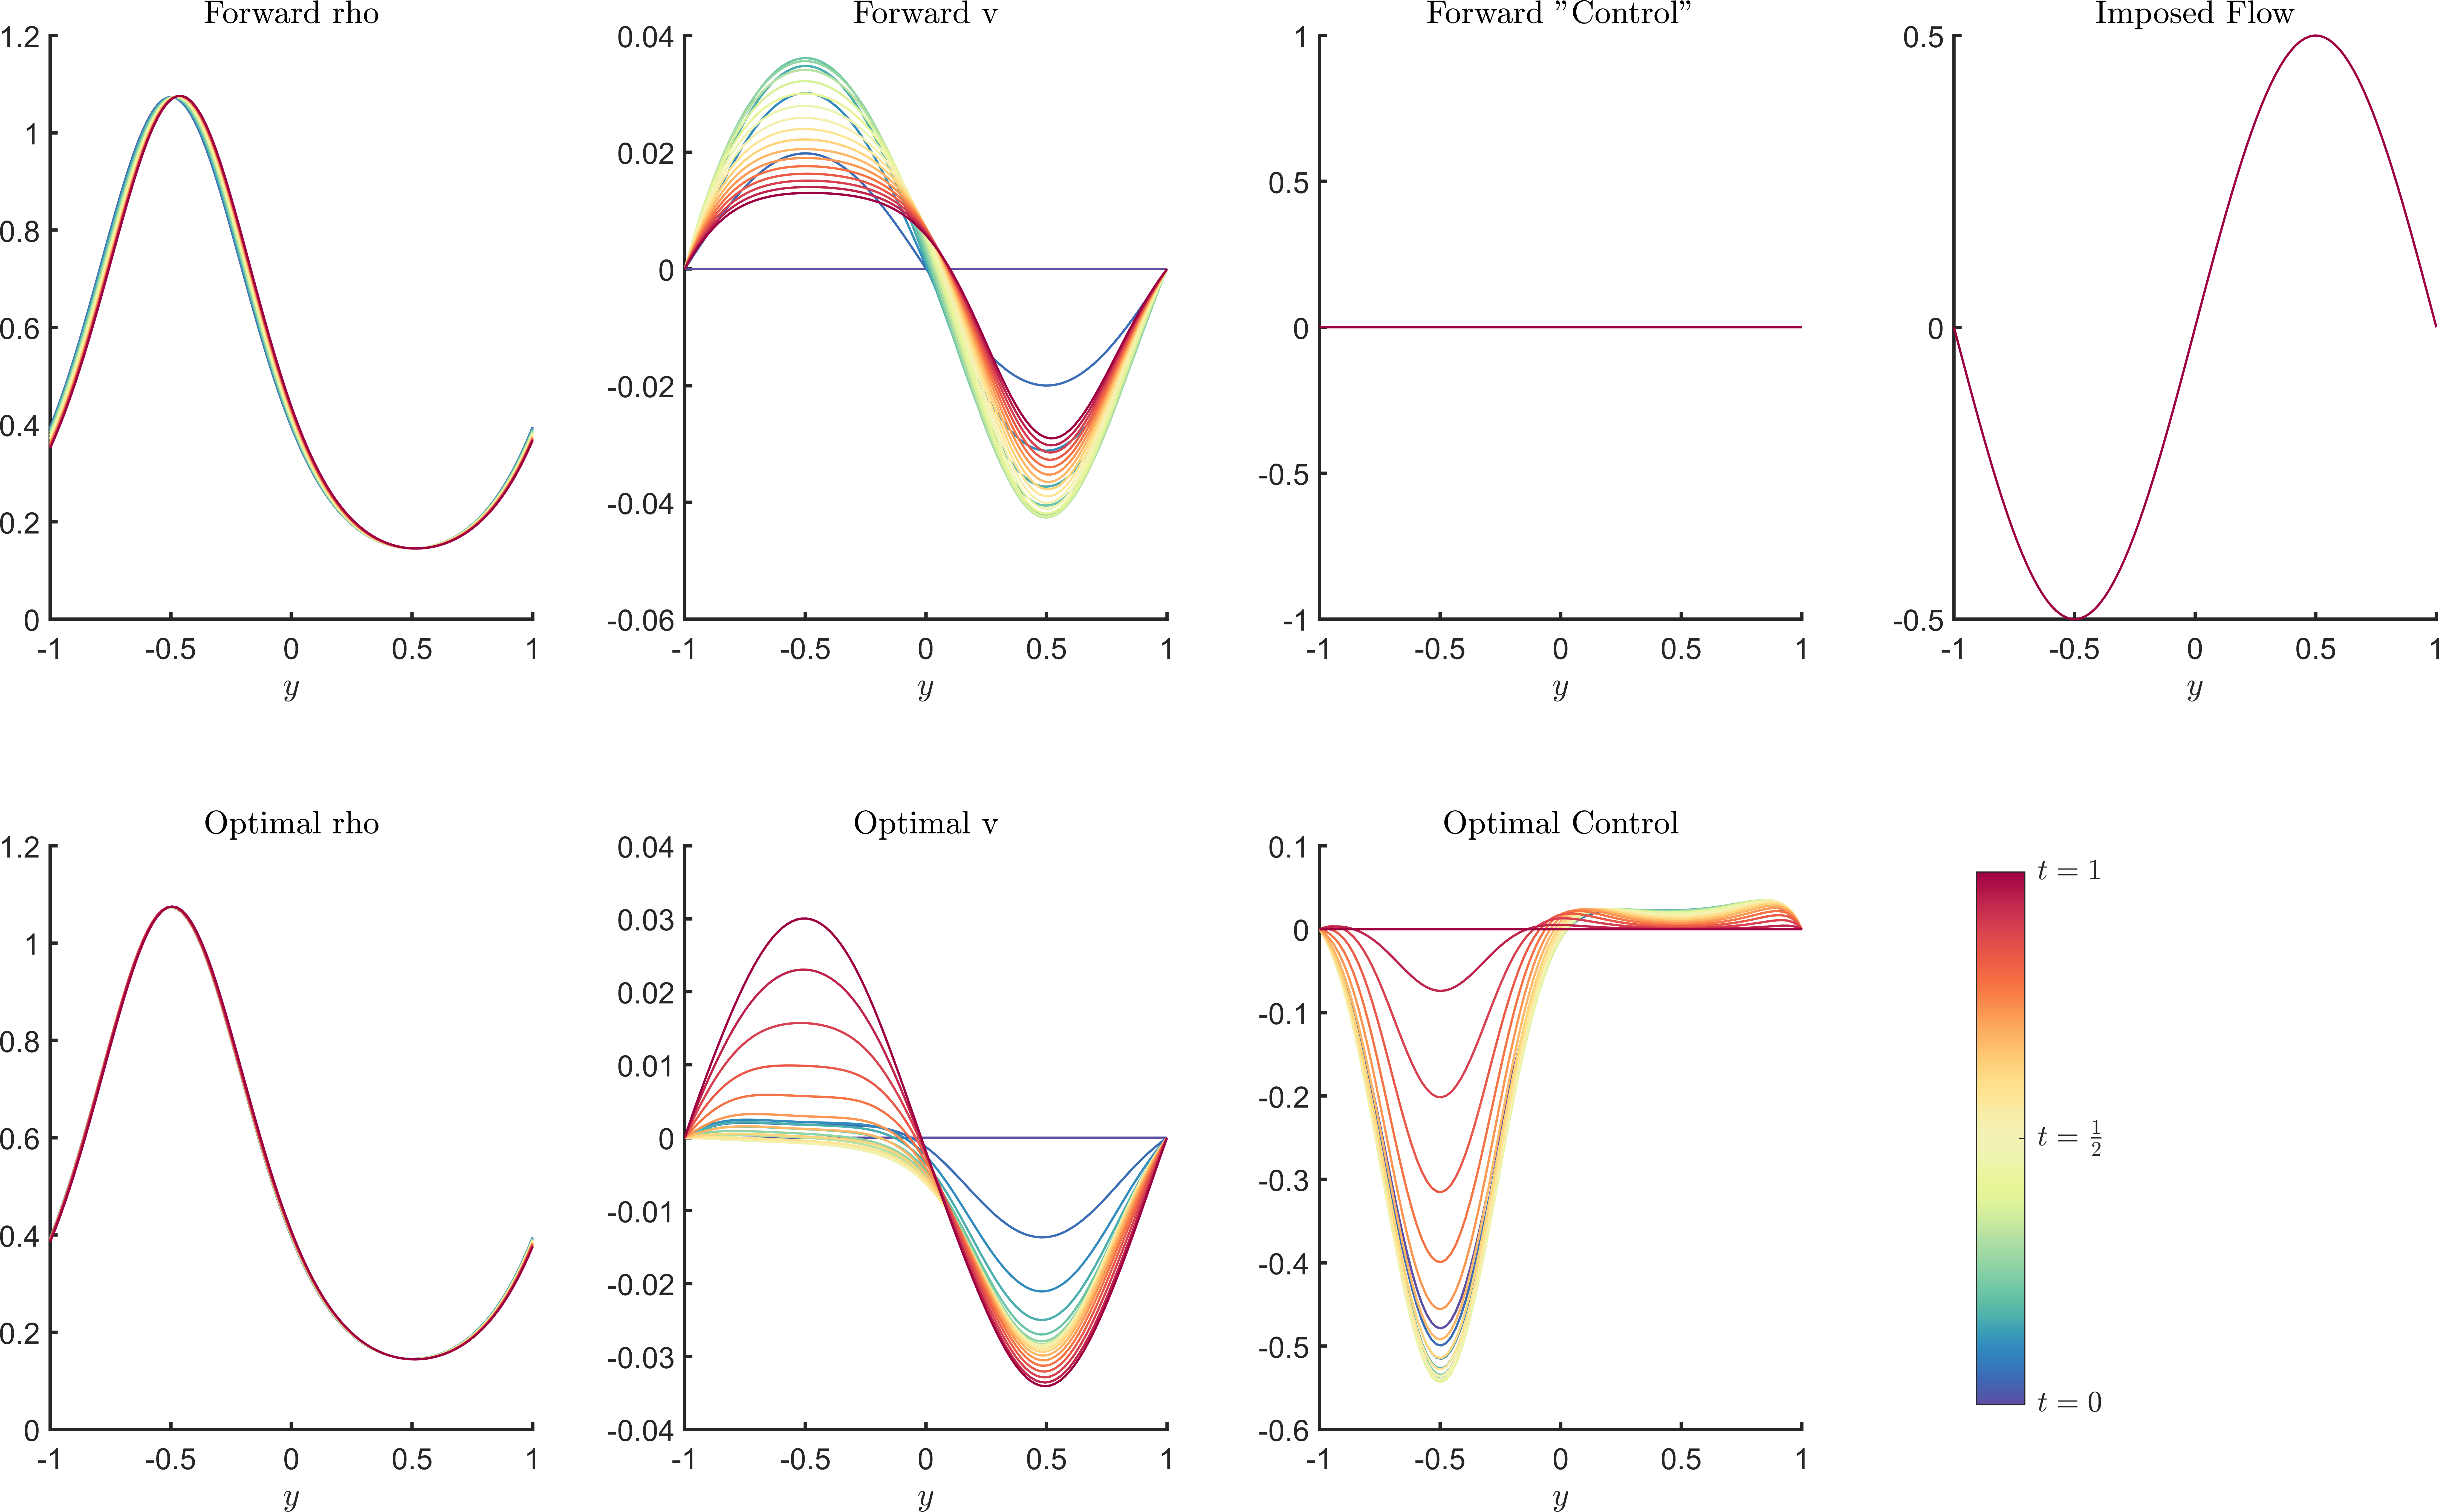
\includegraphics[scale=0.04]{Example1b.png}
		\caption{Example 1, $\eta = 0.1$, $\gamma = 10$, $\kappa = 0$} 
		\label{F3}
	\end{figure}
	
	\section*{Example 2}
	We choose similar configurations as in Example 1, by choosing $\rho_0 = \widehat \rho = c e^{-V{ext}}$:
	\begin{align*}
	&\rho_0 = \widehat \rho = \frac{1}{2.0507} \exp\left(-0.5\left(\frac{2}{3 \pi}\cos\left(\frac{3}{2}\pi y\right)\right) \right)\\
	&\w = \mathbf 0 \\
	&\mathbf{F} = 0.5 \sin(\pi y)\\
	&V_{ext} = 0.5 \left(\frac{2}{3 \pi}\cos\left(\frac{3}{2}\pi \right) \right).
	\end{align*}
	
	We choose $ \beta = 10^{-3}$ and tolerances as in Example 1. Then for $\gamma = 1$, $\eta = 0.1$ and $\kappa = 0$ we get that the problem converges in $517$ iterations. $J_{FW} = 0.0023$, $J_{Opt} = 3.1812 \times 10^{-5}$, see Figure \ref{F4}. We can see that the optimal control tries to cancel out $\mathbf F$ and the optimal $\mathbf v$ is small overall. If we chose $\beta = 10^1$, the algorithm converges in $268$ iterations, but $J_{Opt} =0.0023$ still, since only small amounts of control can be applied.
	Choosing $\kappa = 1$ instead gives $J_{FW} = 2.0588 \times 10^{-4}$ and $J_{Opt} = 9.5725 \times 10^{-6}$. The result can be seen in Figure \ref{F4a}. Again, significant differences in forward solution and optimal control can be observed in comparison to the non-interacting case. 
	Finally, for $\kappa = -1$, we get $J_{FW} = 0.0078$ and $J_{Opt} = 1.0982 \times 10^{-4}$, see Figure \ref{F4b}. Here, the results are relatively similar to the non-interacting problem, but there is a visible difference in the distribution of $\rho$ in the forward problem between non-interacting and attractive particles.
	\\
	For $\gamma = 0.1$, $\eta = 0.01$, and $\kappa = 0$ we get $J_{FW} = 0.0043$, $J_{Opt} = 3.1188 \times 10^{-5}$. For such a  choice of parameters, we can see a difference in the forward problem, since less damping is applied in the system.
	
	
	\begin{figure}[h]
		\centering
		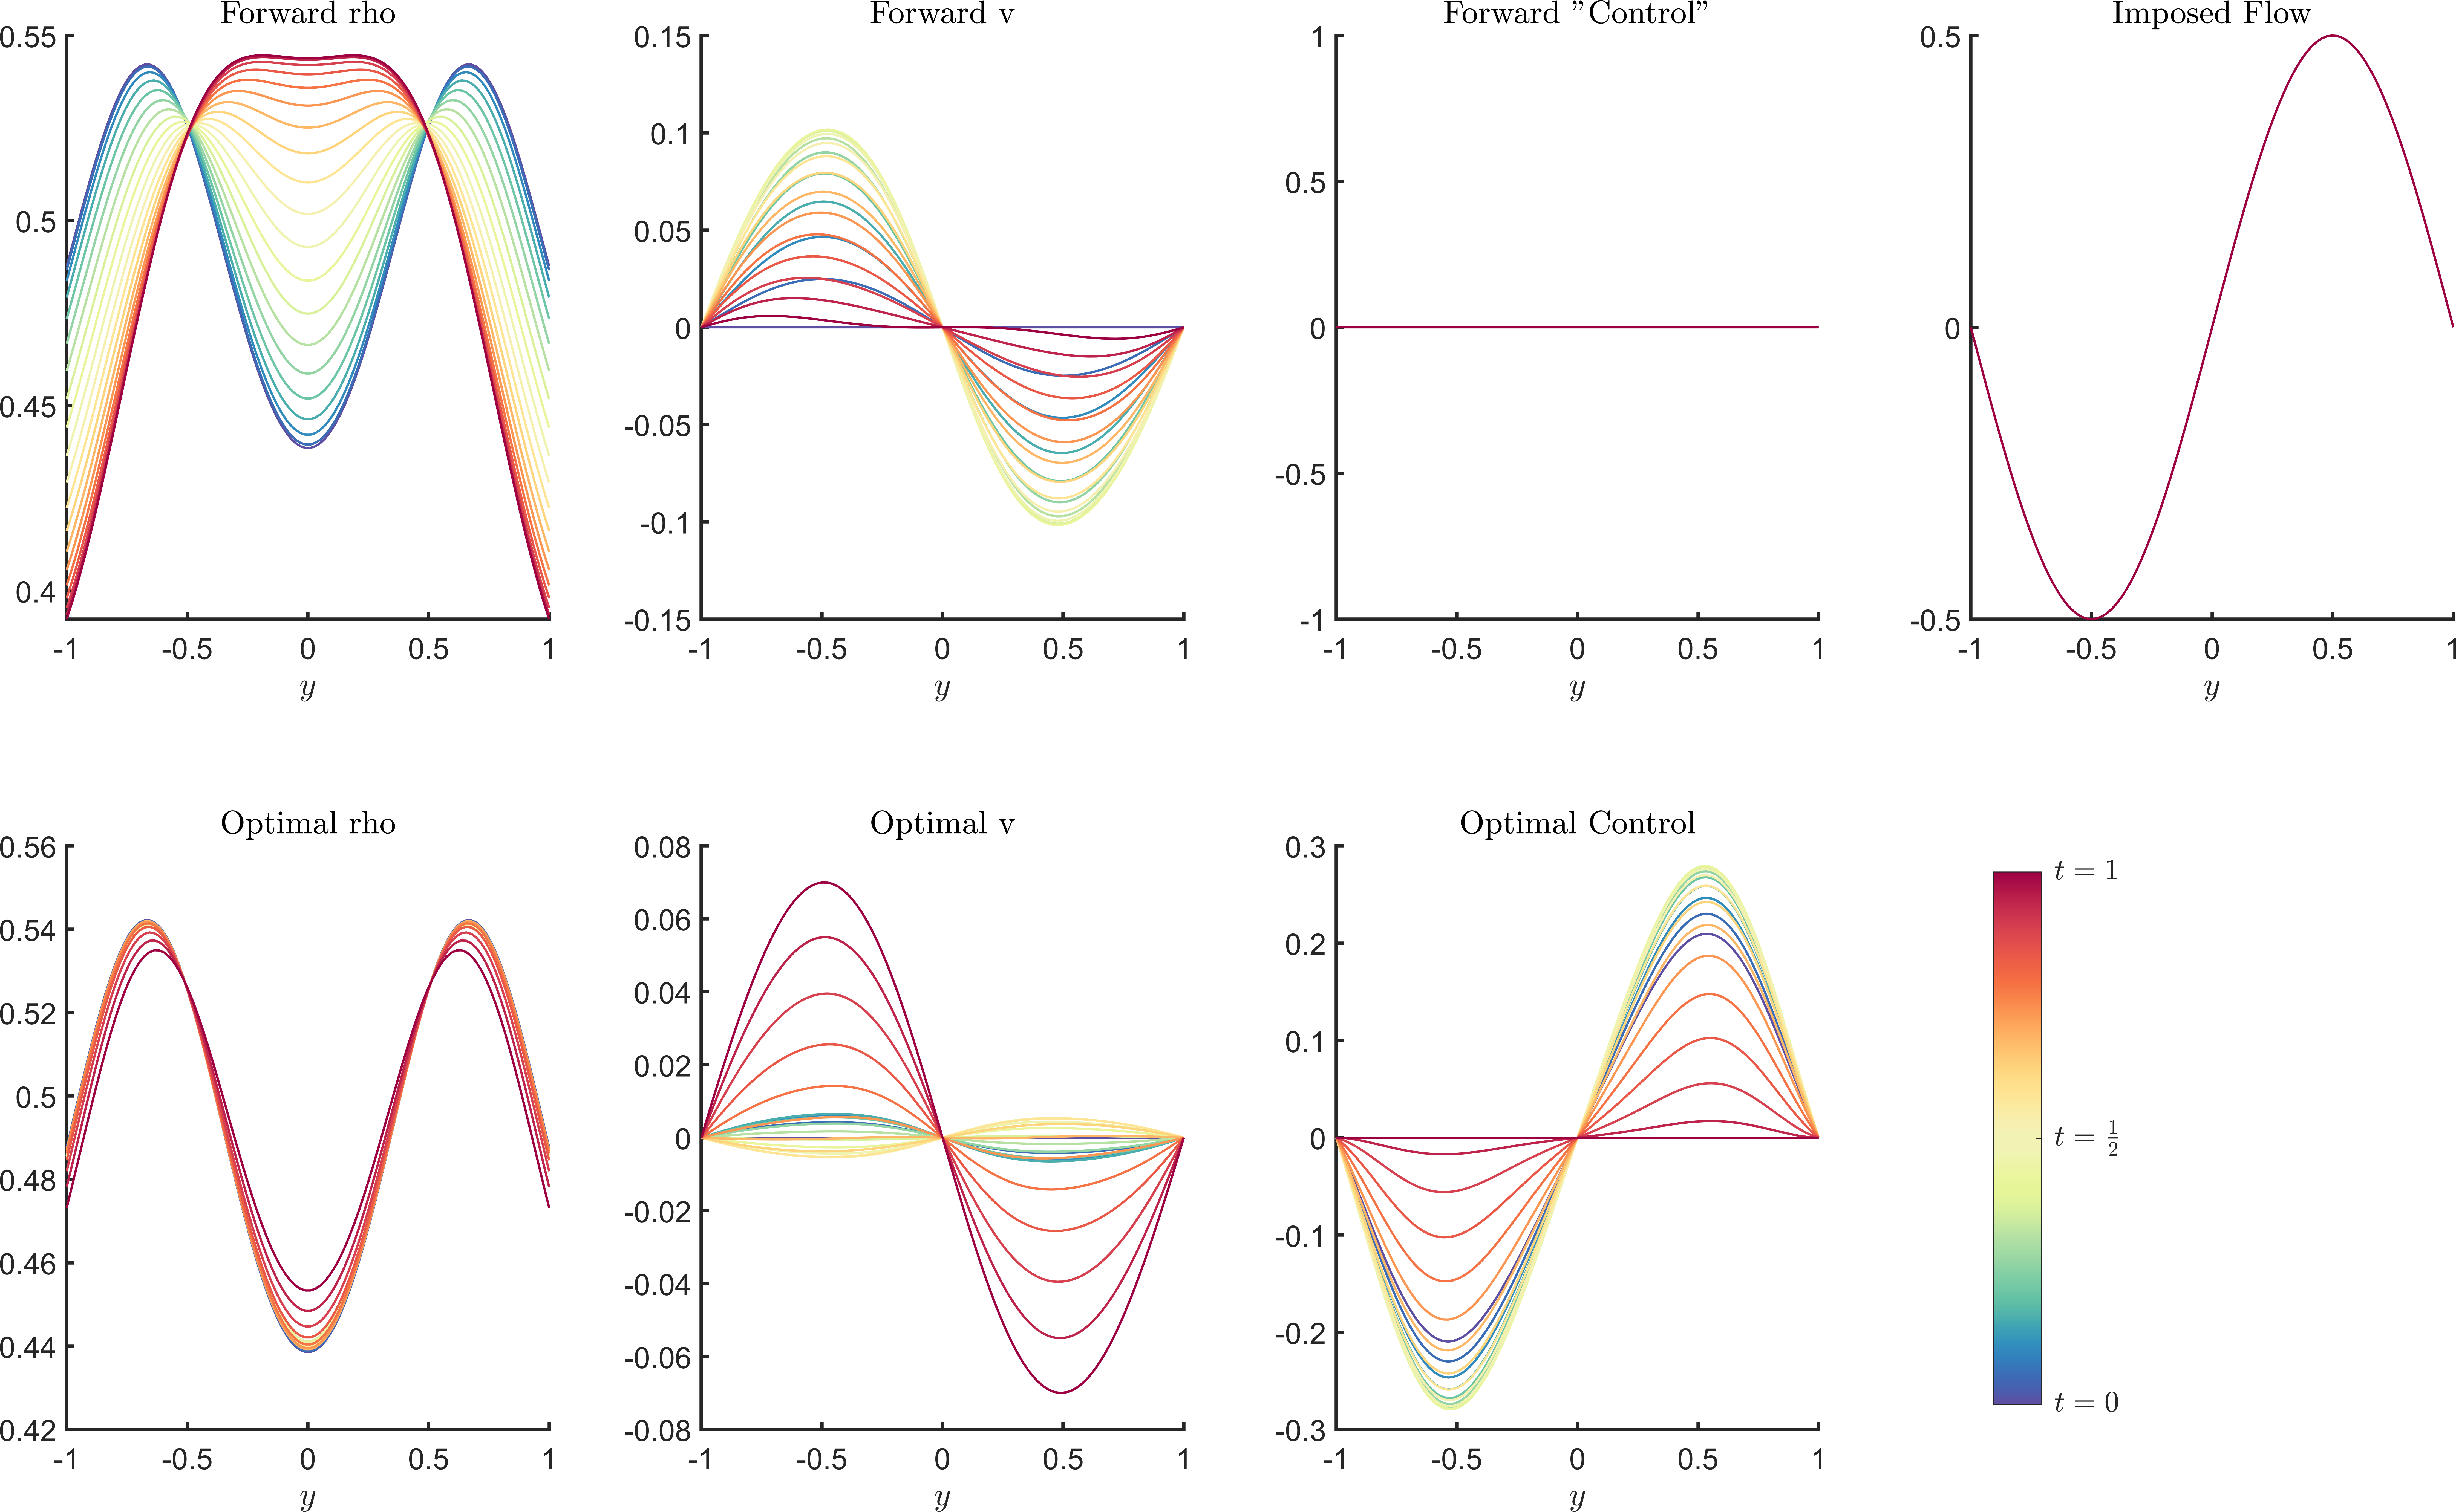
\includegraphics[scale=0.04]{Example2a.png}
		\caption{Example 2, $\eta = 0.1$, $\gamma = 1$, $\kappa = 0$} 
		\label{F4}
	\end{figure}
\begin{figure}[h]
	\centering
	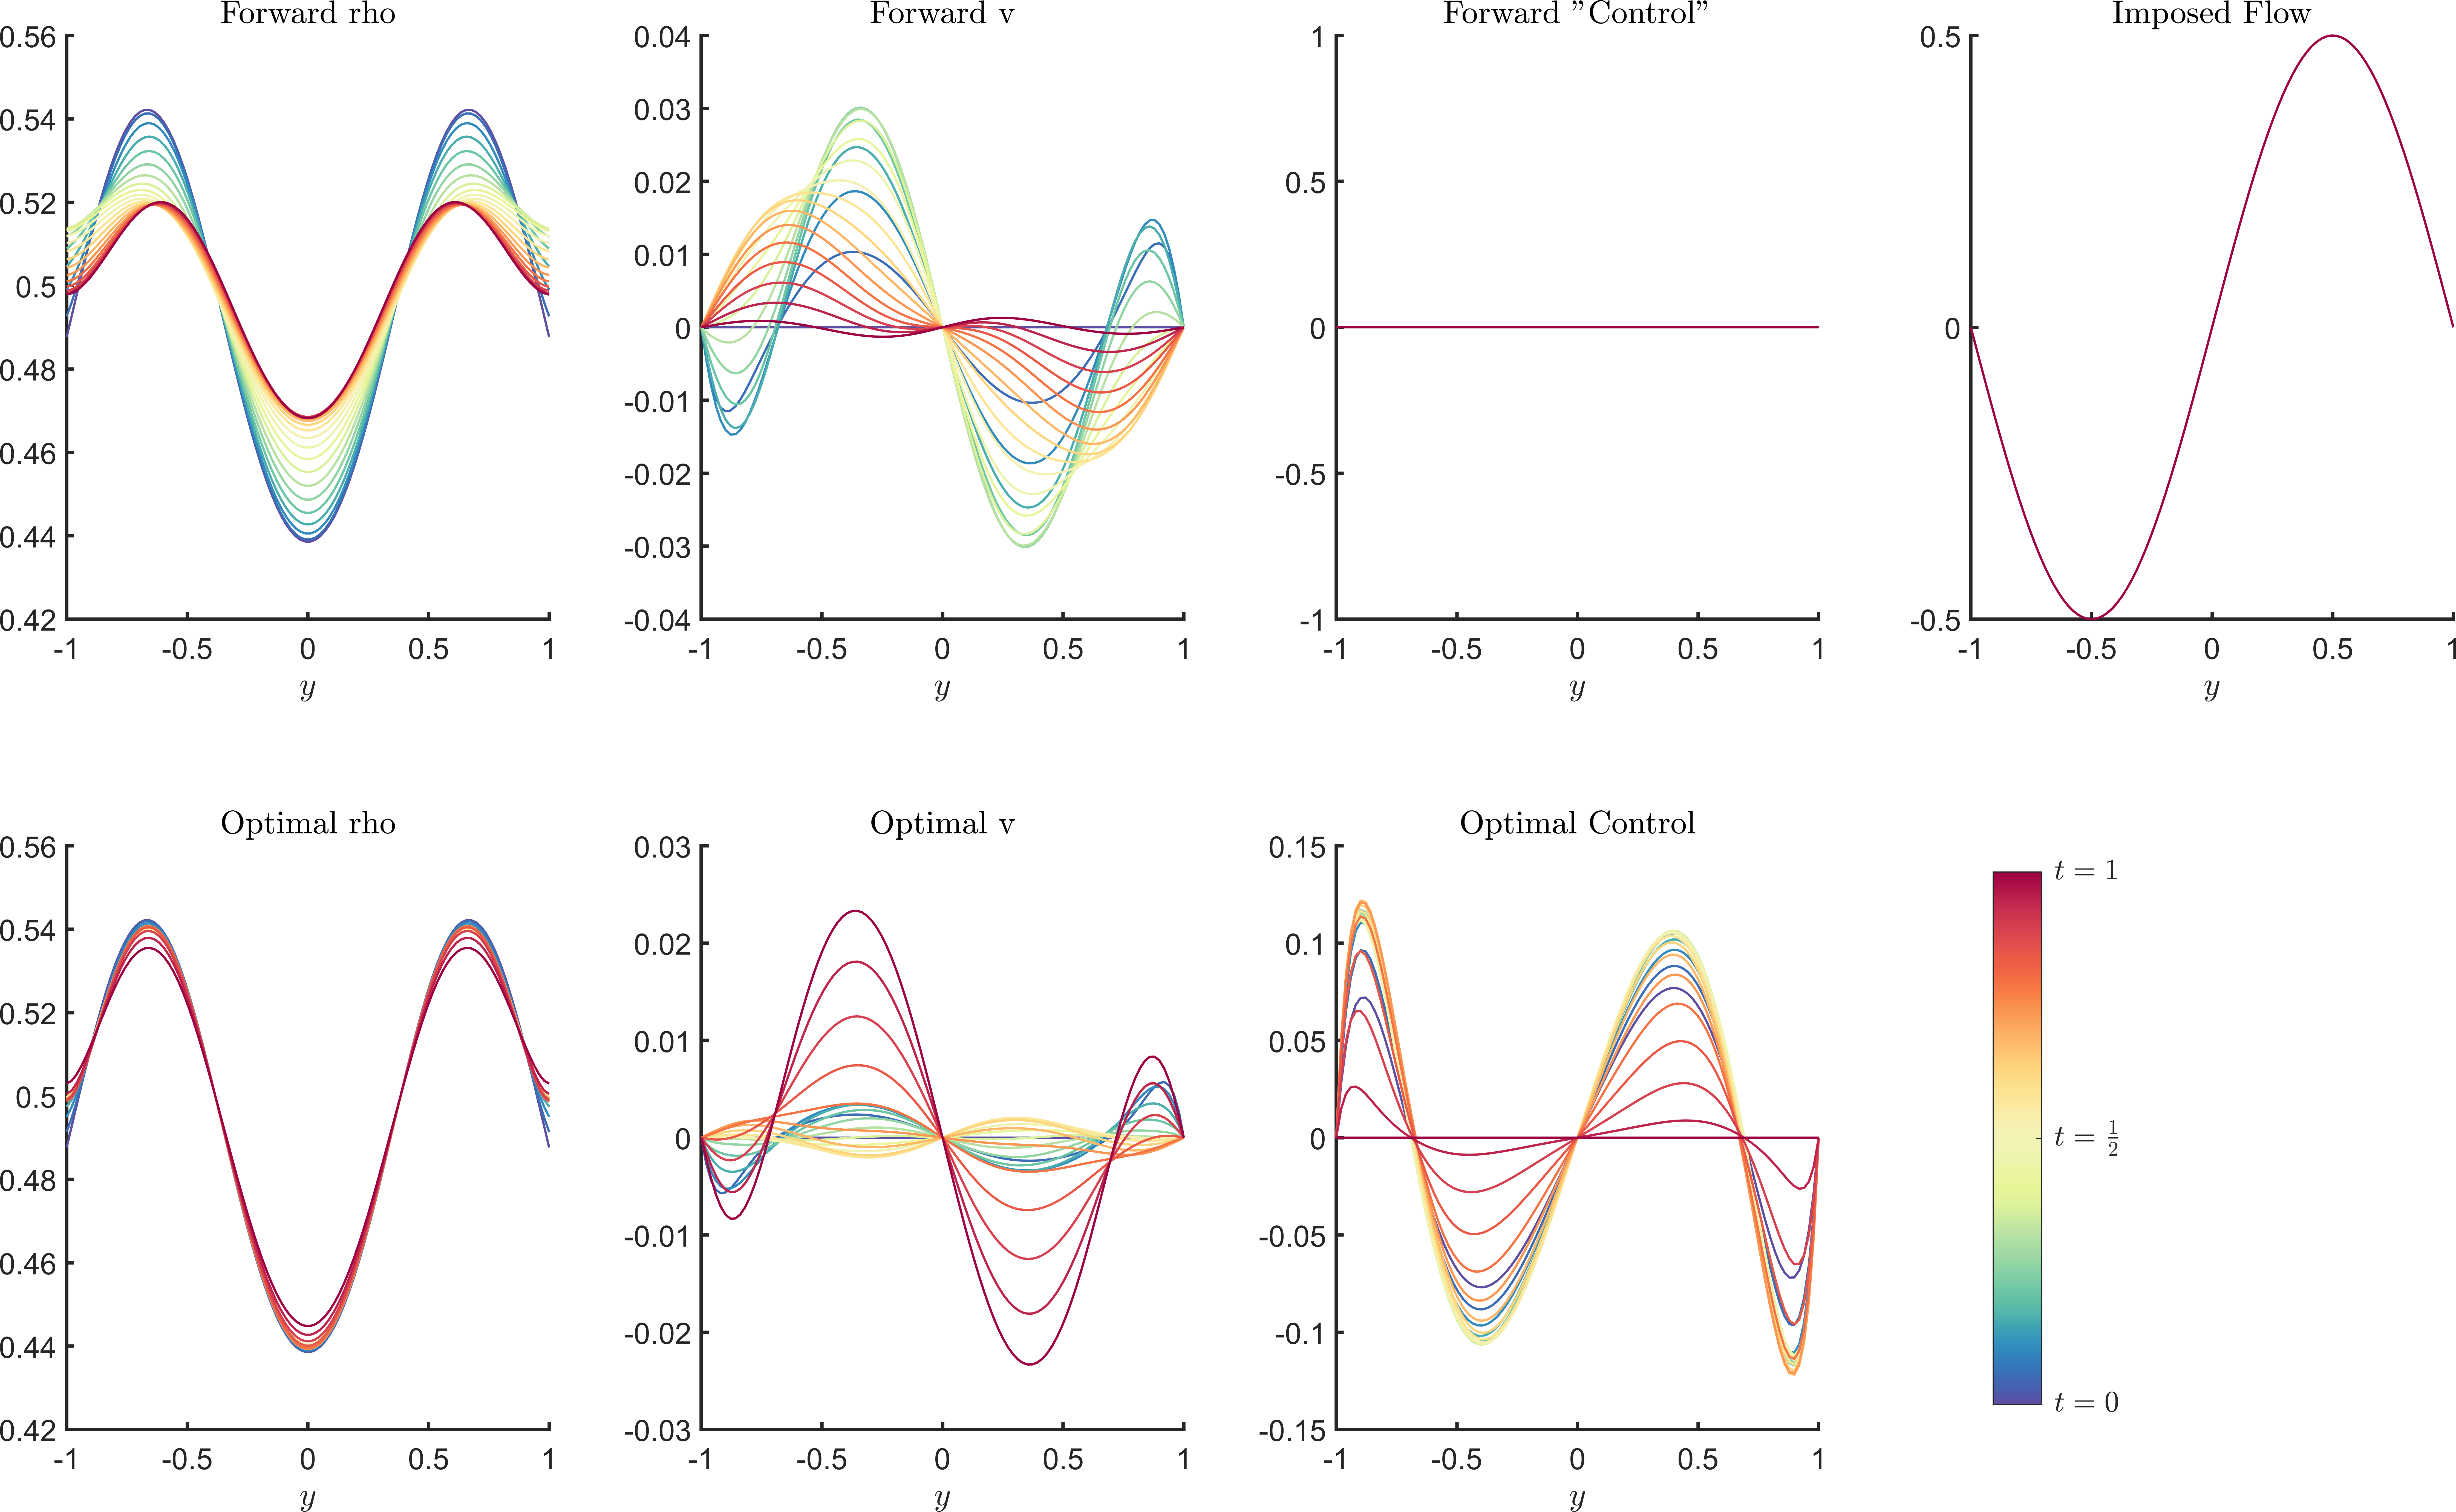
\includegraphics[scale=0.04]{Example211.png}
	\caption{Example 2, $\eta = 0.1$, $\gamma = 1$, $\kappa = 1$} 
	\label{F4a}
\end{figure}
\begin{figure}[h]
	\centering
	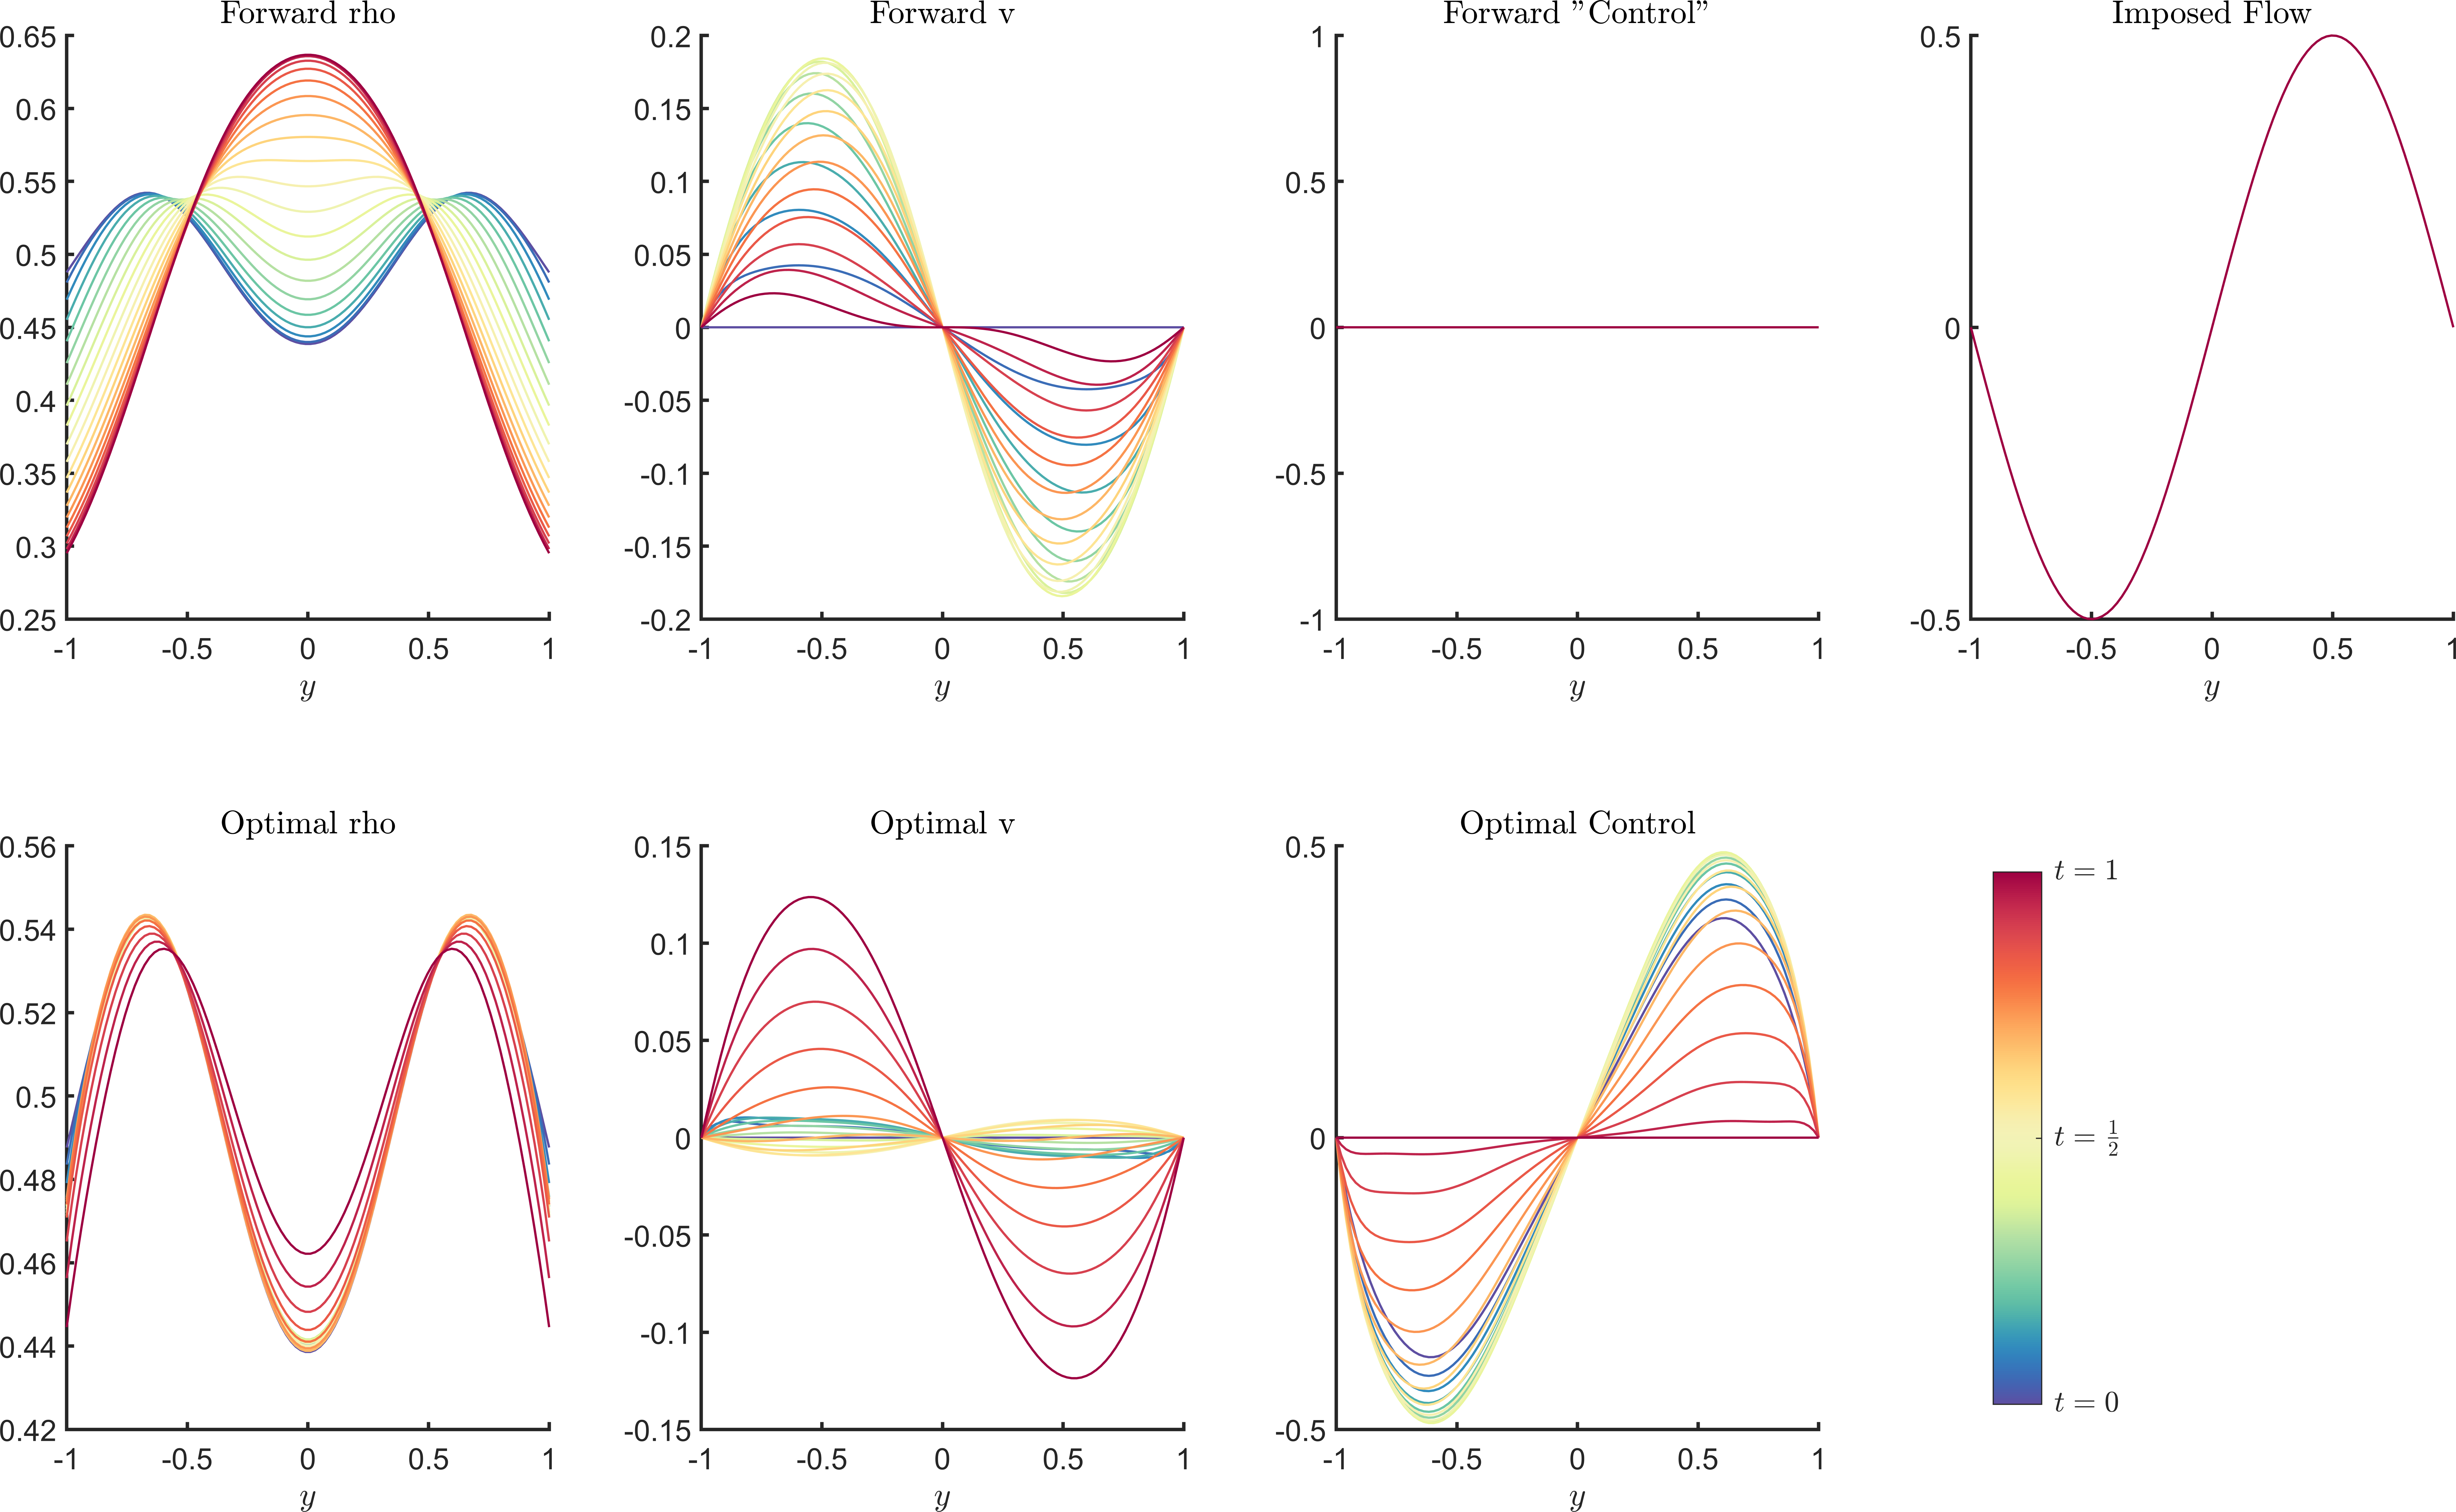
\includegraphics[scale=0.04]{Example21n1.png}
	\caption{Example 2, $\eta = 0.1$, $\gamma = 1$, $\kappa = -1$} 
	\label{F4b}
\end{figure}

	\begin{figure}[h]
		\centering
		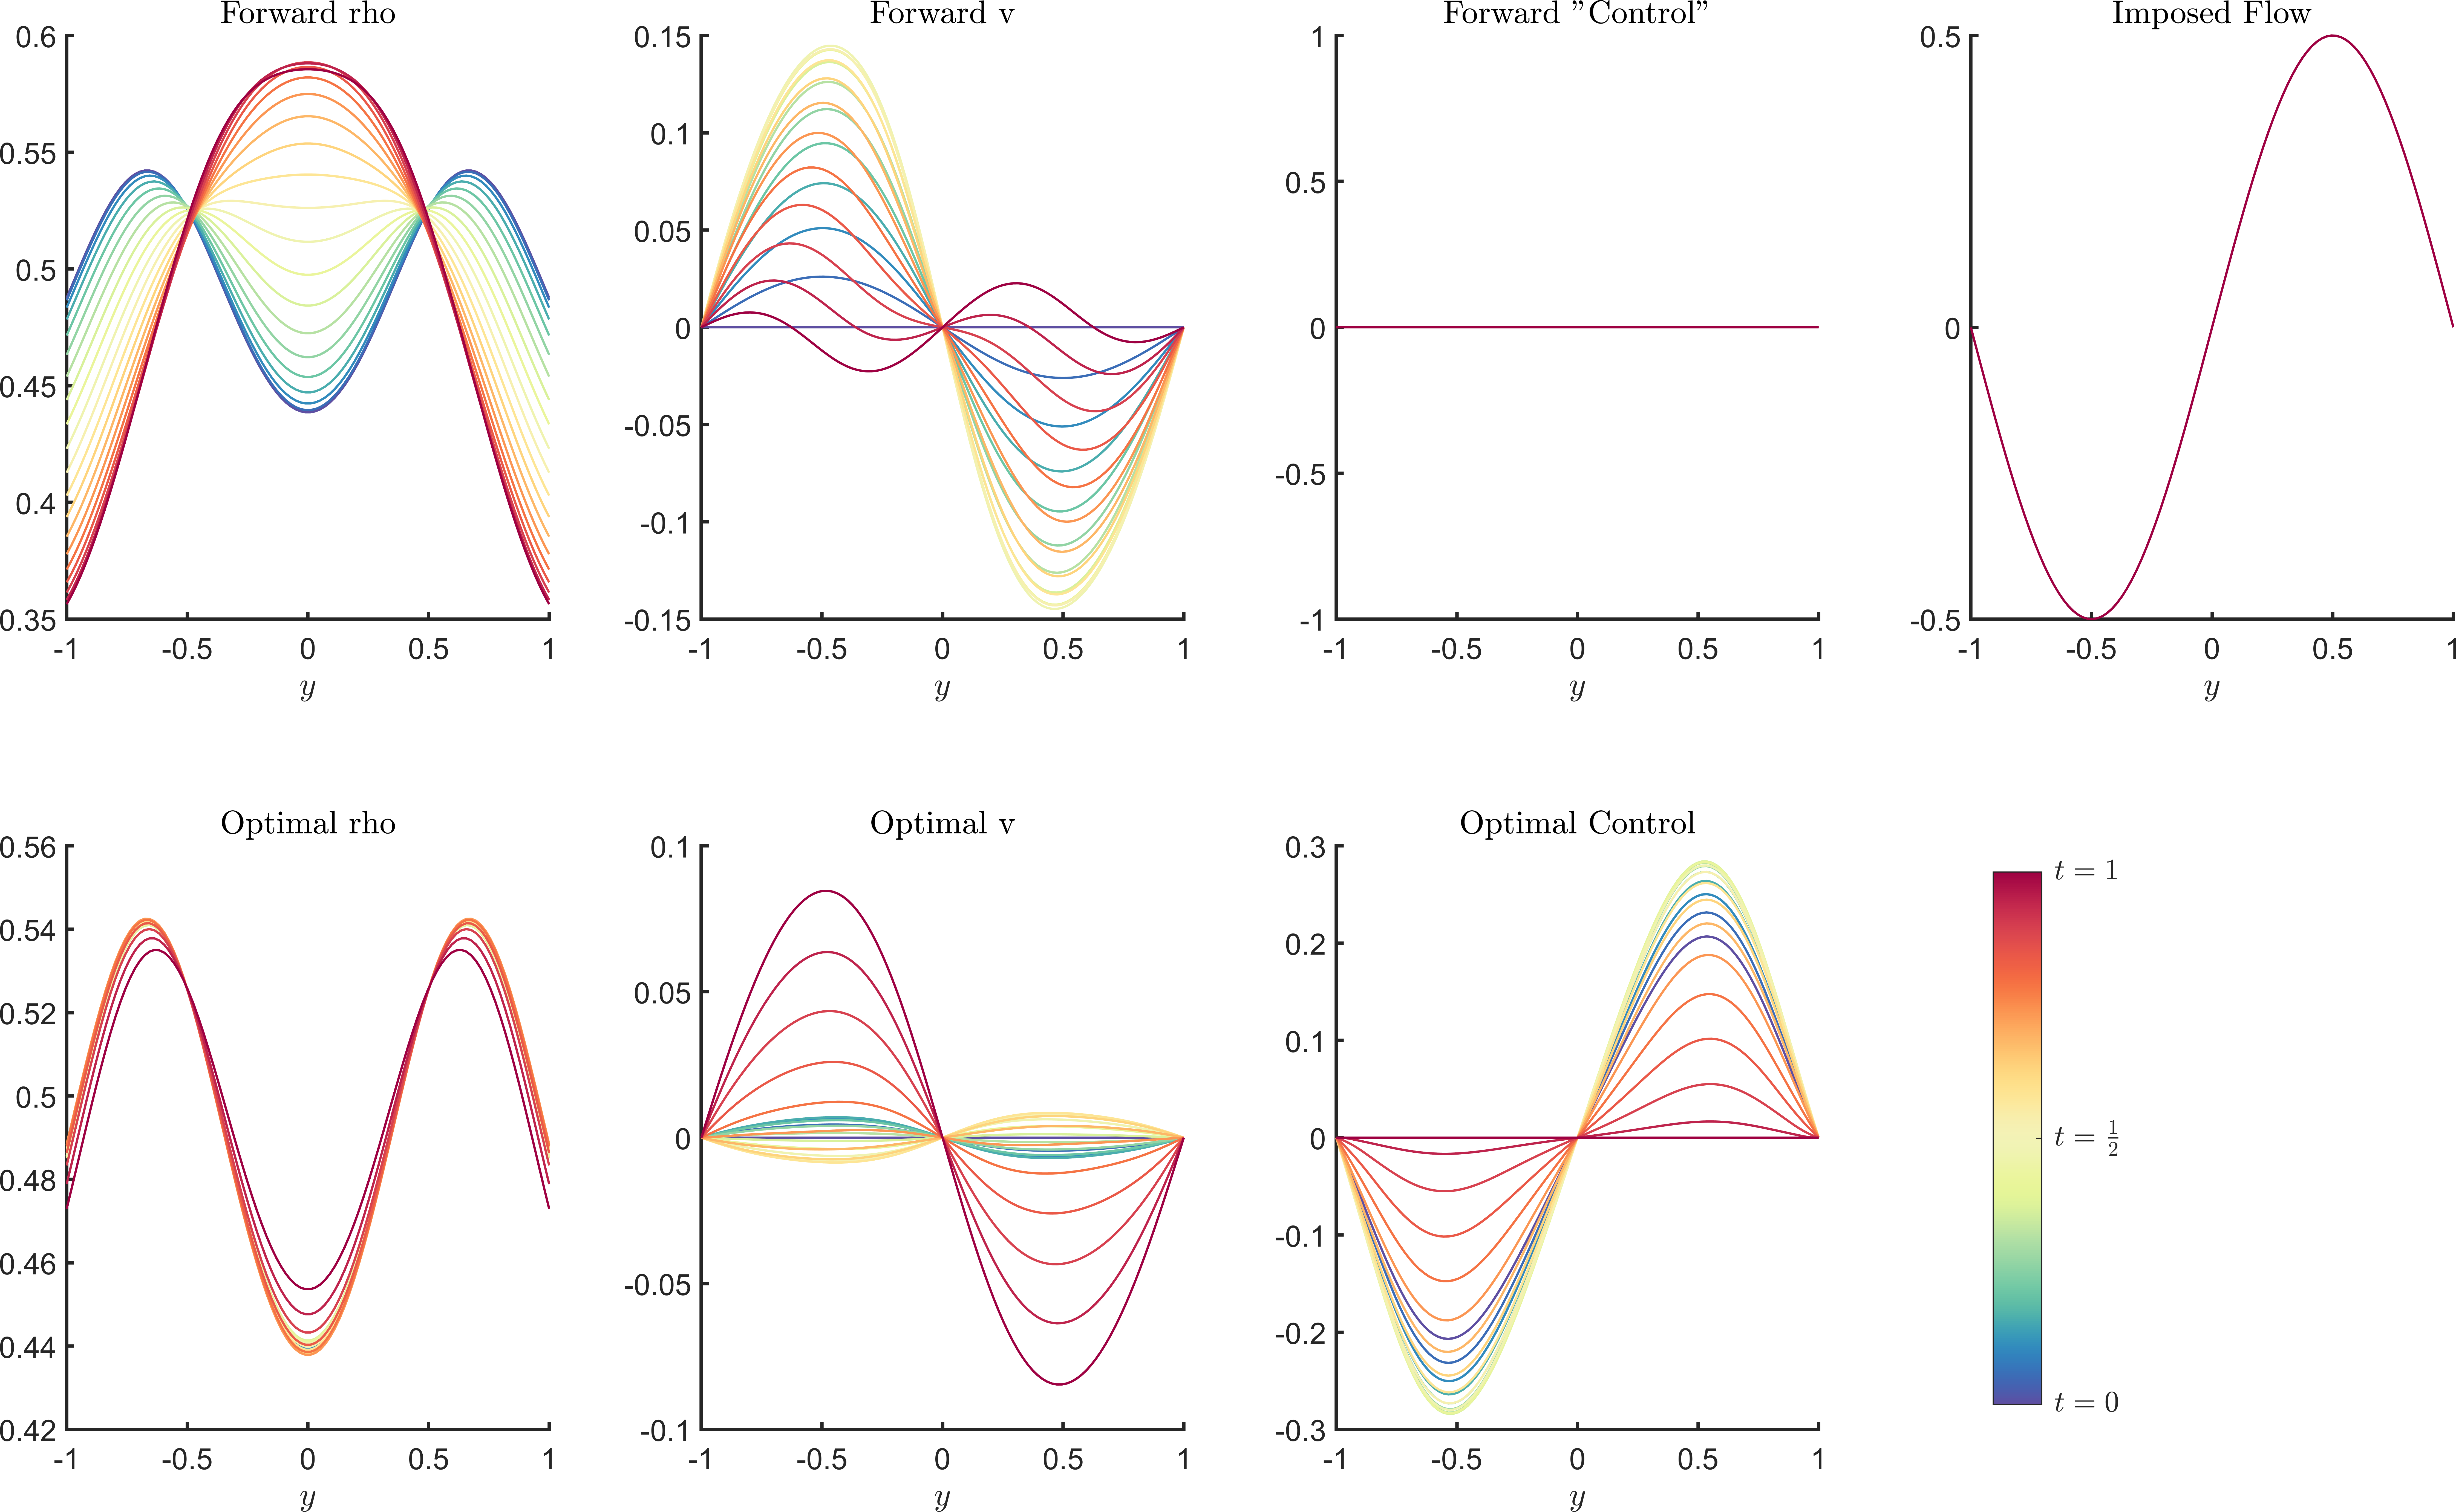
\includegraphics[scale=0.04]{Example2b.png}
		\caption{Example 2, $\eta = 0.01$, $\gamma = 0.1$, $\kappa = 0$} 
		\label{F5}
	\end{figure}

We choose similar configurations as in Example 2, but choosing a different $\rho_0$:
\begin{align*}
&\rho_0 = 1\\
&\widehat \rho = \frac{1}{2.0507} \exp\left(-0.5\left(\frac{2}{3 \pi}\cos\left(\frac{3}{2}\pi y\right)\right) \right)\\
&\w = \mathbf 0 \\
&\mathbf{F} = 0.5 \sin(\pi y)\\
&V_{ext} = 0.5 \left(\frac{2}{3 \pi}\cos\left(\frac{3}{2}\pi \right) \right).
\end{align*}
If we choose $\gamma = 1$, $\eta = 1$, we get $J_{FW} = 0.2522$ and $J_{Opt} = 0.2503$, despite $\beta = 10^{-3}$, showing that this is more difficult. The result can be seen in Figure \ref{F6}. 
Choosing $\eta = 0.1$ gives $J_{FW} 0.2556$, $J_{Opt} = 0.2502$, and Figure \ref{F7} shows that the solution behaves way more erratically without as much smoothing.
\begin{figure}[h]
	\centering
	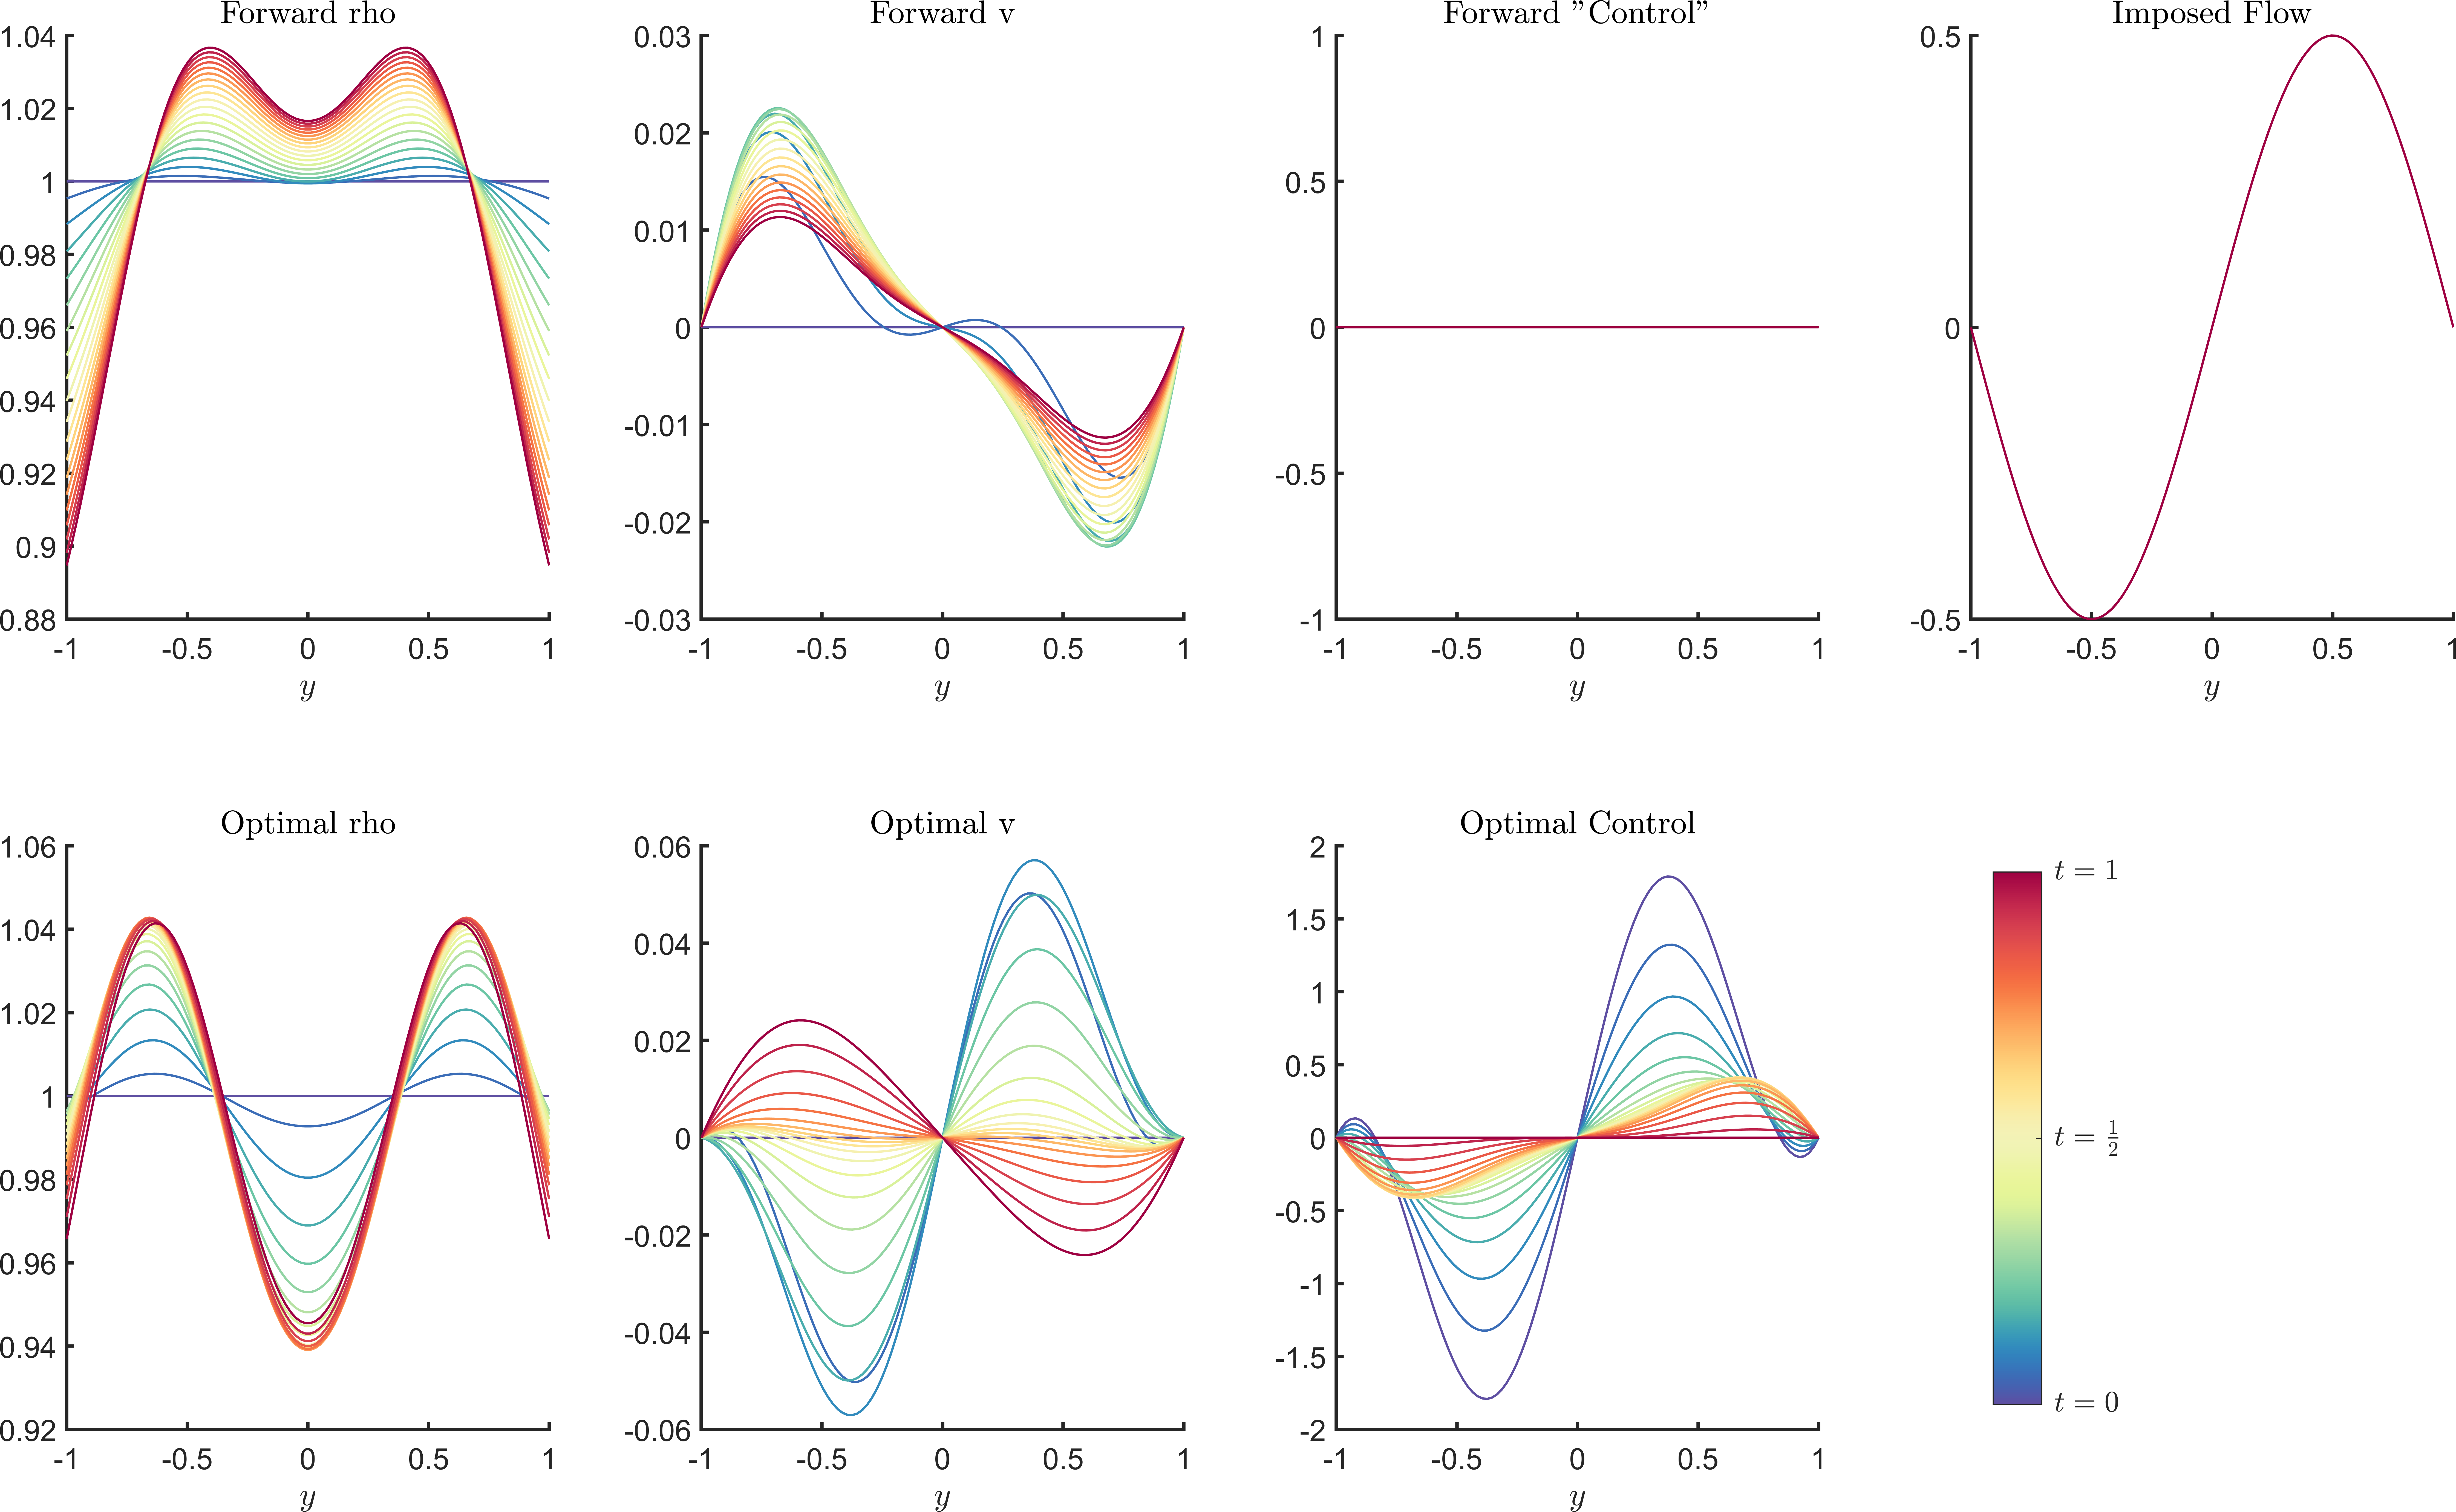
\includegraphics[scale=0.04]{Example3b.png}
	\caption{Example 3, $\eta = 1$, $\gamma = 1$, $\kappa = 0$} 
	\label{F6}
\end{figure}

\begin{figure}[h]
	\centering
	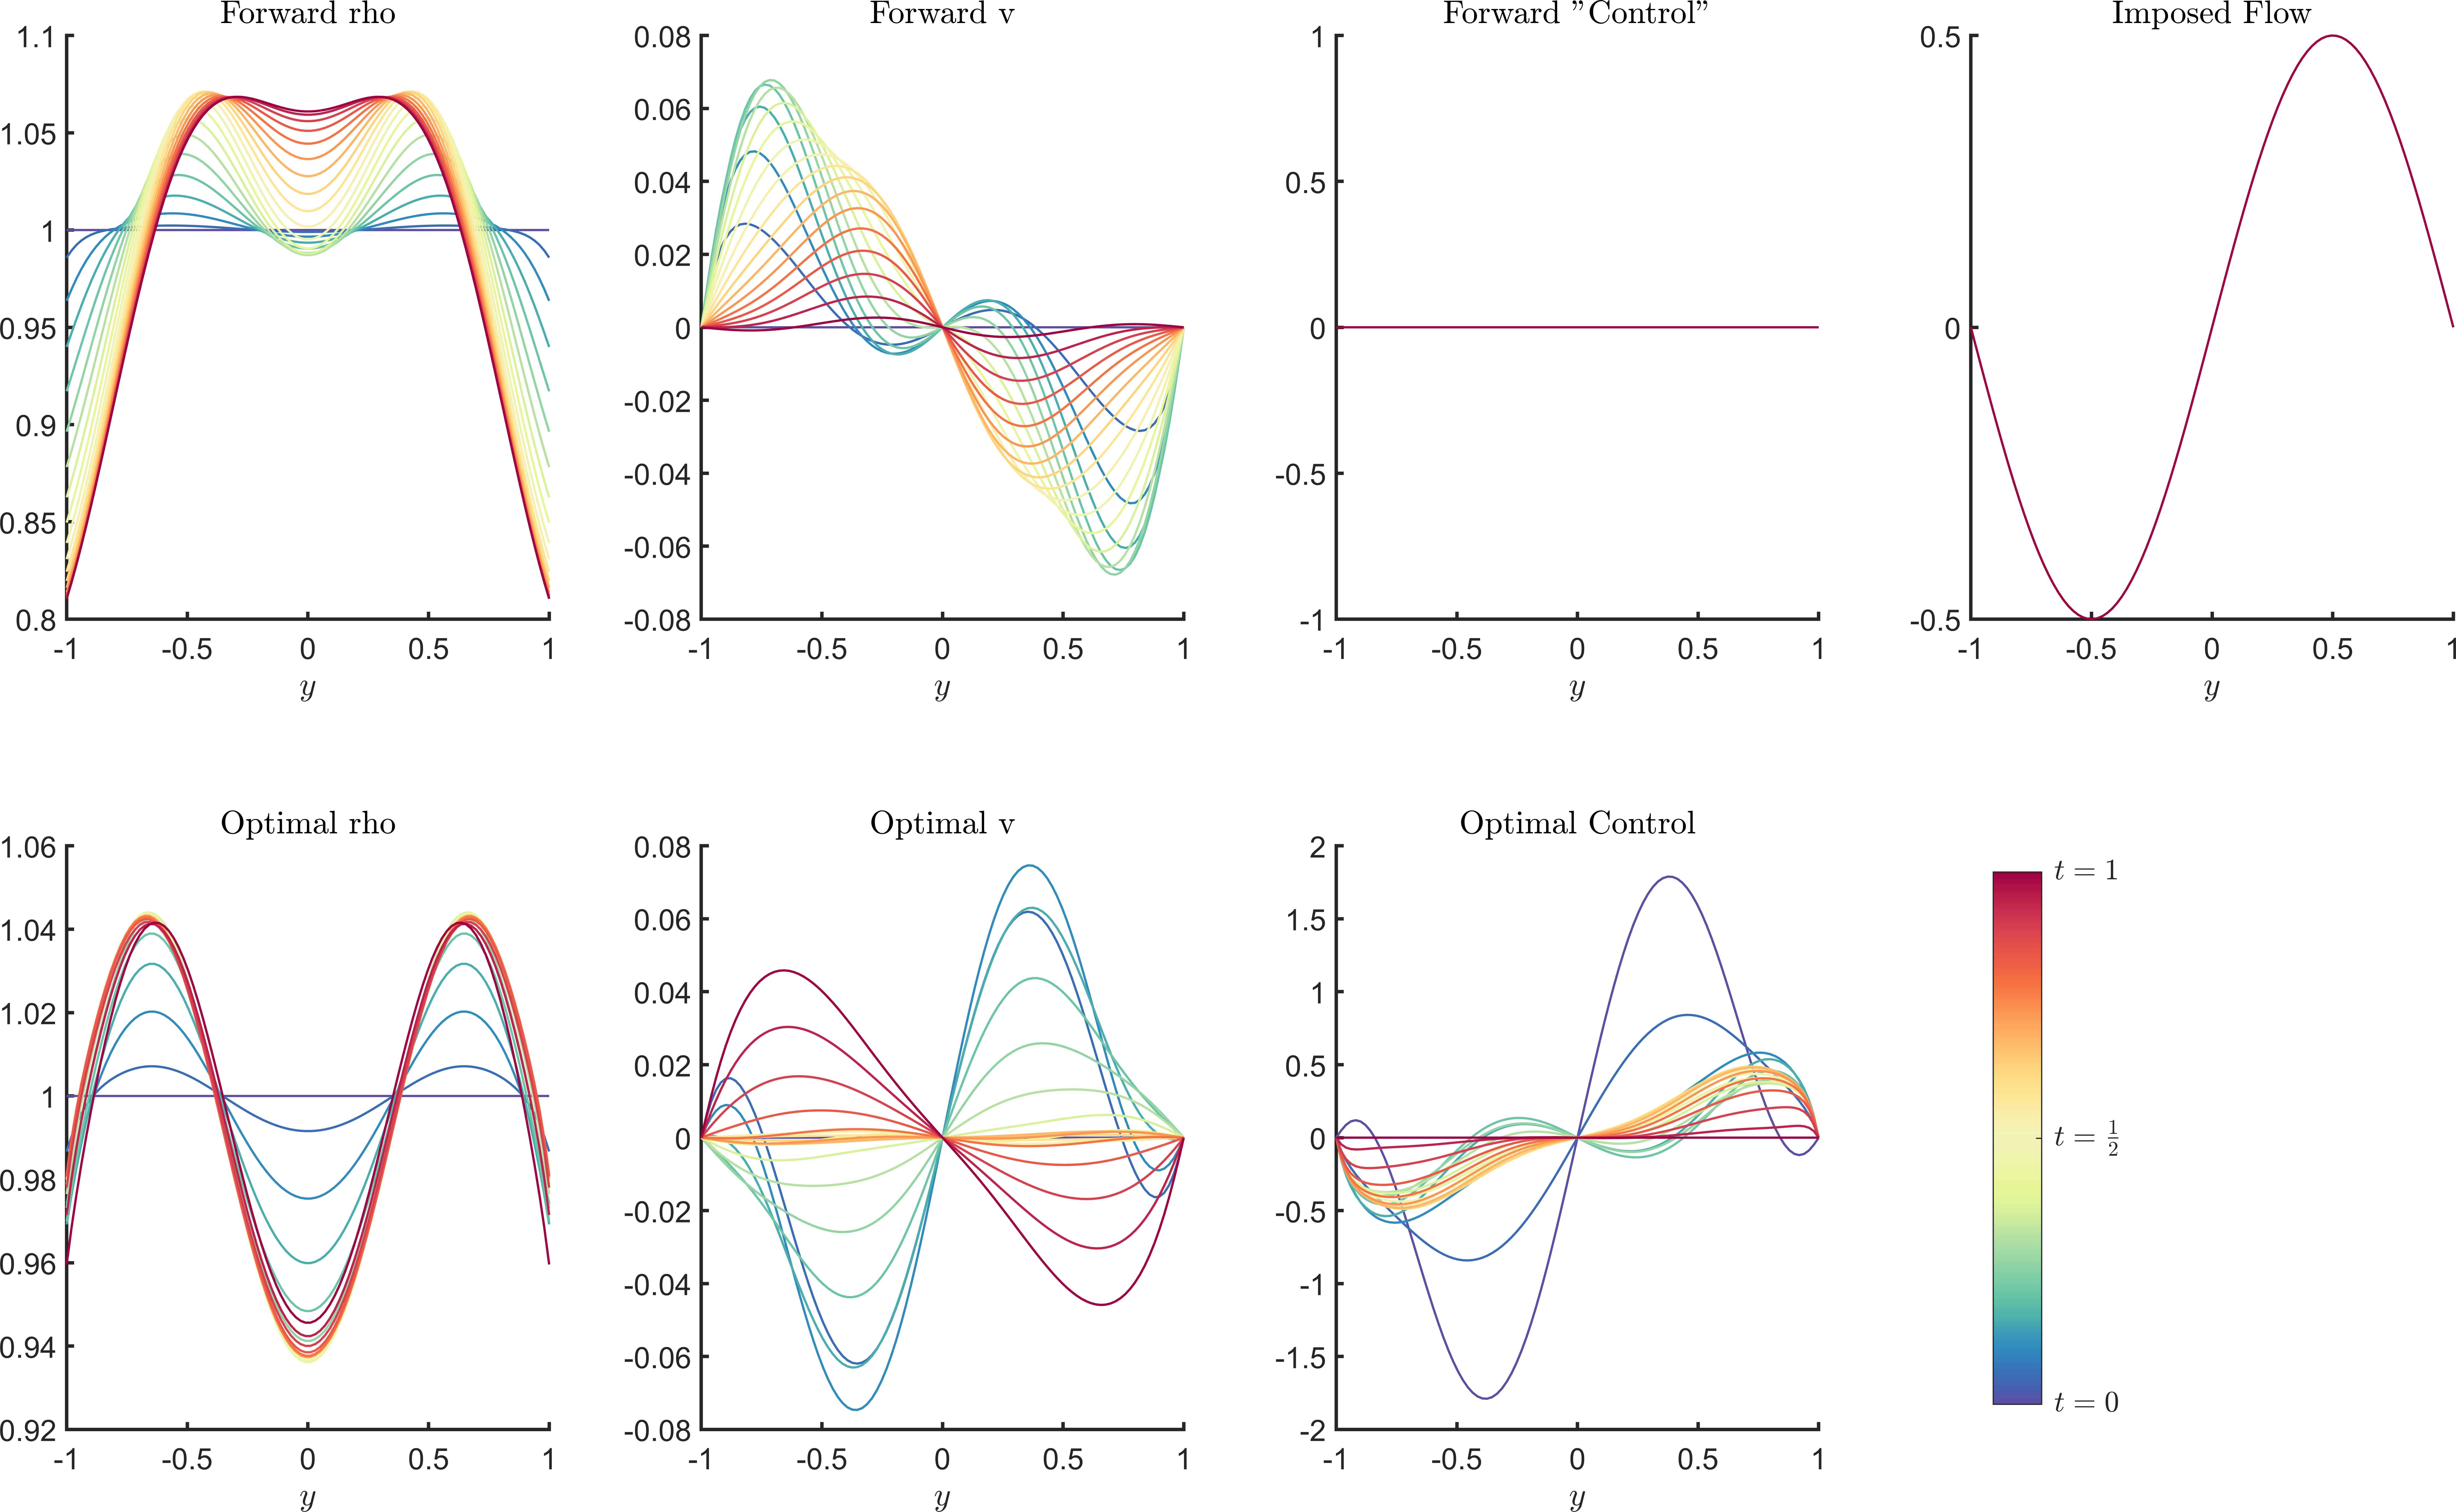
\includegraphics[scale=0.04]{Example3a.png}
	\caption{Example 3, $\eta = 0.1$, $\gamma = 1$, $\kappa = 0$} 
	\label{F7}
\end{figure}
\end{document}